\documentclass[12pt]{article}
\usepackage[english]{babel}
\usepackage[utf8x]{inputenc}
\usepackage{amsmath}
\usepackage{graphicx}
\usepackage[table,xcdraw]{xcolor}
\usepackage[colorinlistoftodos]{todonotes}
\usepackage[hidelinks, breaklinks]{hyperref}
\usepackage{multirow}
\usepackage{caption}
\usepackage{float}

\usepackage{titlesec}  
\setcounter{tocdepth}{4}
\setcounter{secnumdepth}{4}
\titleformat{\paragraph}
{\normalfont\normalsize\bfseries}{\theparagraph}{1em}{}
\titlespacing*{\paragraph}
{0pt}{3.25ex plus 1ex minus .2ex}{1.5ex plus .2ex}

\begin{document}

\begin{titlepage}

\newcommand{\HRule}{\rule{\linewidth}{0.5mm}} % Defines a new command for the horizontal lines, change thickness here

%----------------------------------------------------------------------------------------

\center % Center everything on the page
 
%----------------------------------------------------------------------------------------
%	HEADING SECTIONS
%----------------------------------------------------------------------------------------

\textsc{\LARGE Università degli studi di Milano-Bicocca}\\[1cm] % Name of your university/college\n textsc{\Large Sistemi Complessi: Modelli e Simulazione}\\[0.3cm] % Major heading such as course name
\textsc{\large Final Project}\\[0.1cm] % Minor heading such as course title

%----------------------------------------------------------------------------------------
%	TITLE SECTION
%----------------------------------------------------------------------------------------

\HRule \\[0.4cm]
{ \LARGE \bfseries Automatic Guided Vehicle System for warehouse management: implementation and simulation}\\[0.4cm] % Title of your document
\HRule \\[1.5cm]
 
%----------------------------------------------------------------------------------------
%	AUTHOR SECTION
%----------------------------------------------------------------------------------------

\large
\emph{Authors:}\\
Andrea Spreafico - 793317 - a.spreafico13@campus.unimib.it \\   % Your name
Francesco Prete - 793389 - f.prete4@campus.unimib.it   \\[2cm] % Your name

%----------------------------------------------------------------------------------------
%	LOGO SECTION
%----------------------------------------------------------------------------------------


\includegraphics{logo.png}\\[1cm] % Include a department/university logo - this will require the graphicx package
 
%----------------------------------------------------------------------------------------

\vfill % Fill the rest of the page with whitespace
\end{titlepage}


\renewcommand{\contentsname}{Contenuti}
\renewcommand\listfigurename{Lista delle figure}
\renewcommand\listtablename{Lista delle tabelle}

\tableofcontents

\newpage

\listoffigures
\listoftables



\newpage 
%%%%%%%%%%%%%%%%%%%%%%%%%%%%%%%%%%%%%%%%%%%%%%%
% Introduzione al problema
%%%%%%%%%%%%%%%%%%%%%%%%%%%%%%%%%%%%%%%%%%%%%%%
\section{Introduzione al problema} % Main chapter title
\subsection{Panoramica}
IoT, guida autonoma, domotica e tutto quello che riguarda l’automazione di processi (produttivi e domestici) attraverso l’uso di “macchine intelligenti” sono argomenti sempre più presenti nella vita di tutti i giorni e sono destinati, in un futuro molto vicino, ad essere la normalità.

\noindent Questo è l’ambito in cui si sviluppa il nostro progetto: l’automazione dei processi produttivi di un’azienda di trasporti e logistica, la LDE S.r.l. di Brembate. Questa società ci ha fornito i dati riguardanti la gestione tecnica, gli ordini e il magazzino e, quindi, tutti i dati utilizzati per lo sviluppo di questo lavoro sono reali e derivati dalla sopracitata azienda.
Ad oggi, in LDE lo smistamento dei pacchi è eseguito in maniera totalmente manuale dai dipendenti e questo prevede un grande sforzo lavorativo ed organizzativo.

\subsection{Obiettivi}
Lo scopo di questo lavoro è quello di implementare, simulare e valutare la realizzazione di un sistema a veicoli a guida autonoma per la gestione semi automatica di un magazzino.
In particolare, lo scopo finale del lavoro sarà quello di stimare il numero ottimale di veicoli e il comportamento che questi ultimi dovranno adottare per minimizzare i costi e i tempi di esecuzione nello smistamento degli ordini.

\subsection{Strumenti utilizzati}
Gli strumenti principali utilizzati per la progettazione e l'implementazione di questo lavoro sono stati:
\begin{itemize}
\item Python 3.6.7 \cite{Python}
\item PycxSimulator \cite{PycxSimulator}
\item Tableau \cite{Tableau} 
\item Github \cite{GitHub}
\end{itemize}

\newpage
%%%%%%%%%%%%%%%%%%%%%%%%%%%%%%%%%%%%%%%%%%%%%%%
% Stato dell'arte
%%%%%%%%%%%%%%%%%%%%%%%%%%%%%%%%%%%%%%%%%%%%%%%
\section{Stato dell'arte}

\subsection{Agente}

Un agente è una qualunque entità in grado di percepire l’ambiente che lo circonda attraverso l’uso di sensori e di eseguire delle azioni attraverso degli attuatori. Ad esempio, in un essere umano alcuni sensori sono gli occhi e le orecchie. Gli attuatori possono essere le mani, i piedi o pi`u in generale i muscoli.

\begin{figure}[ht]
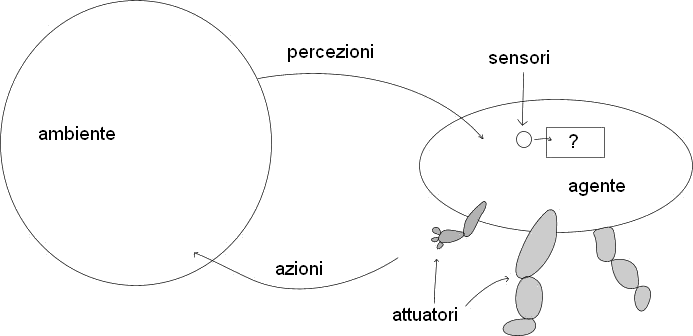
\includegraphics[width=\textwidth,height=\textheight,keepaspectratio]{Figures/Vario/Agente.png}
\caption[Interazione di un agente con l'ambiente esterno]{Interazione di un agente con l'ambiente esterno}
\label{fig:Agente}
\end{figure}

Nel campo dell’Intelligenza artificiale un obiettivo fondamentale è la realizzazione di agenti intelligenti (o agenti razionali). Nella fattispecie un agente si definisce intelligente se fa la cosa giusta al momento giusto. \\
Per poter stabilire questo, però, occorre fornire una qualche misura delle prestazioni e definire come e quando eseguire la valutazione. Inoltre, questo rende necessario un modello di successo, stabilito a priori, con il quale confrontare i risultati ottenuti. \cite{AgenteIntelligente}

\label{Agente}
\begin{itemize}
\item agenti con riflessi semplici (detti anche puramente reattivi);
\item agenti con riflessi basati su modello;
\item agenti basati su obiettivo;
\item agenti basati su utilità;
\item agenti che apprendono;
\end{itemize}

\noindent Per questo lavoro andremo a considerare agenti basati su obiettivo, ovvero agenti con uno stato interno e che memorizzano informazioni per permettergli di raggiungere il proprio obiettivo. 

\subsection{Sistema}
Prima di comprendere il termine "sistema complesso" bisogna andare a capire cos'è un sistema. Esistono varie definizioni di questo termine, che dipendono principalmente dal contesto in cui viene utilizzato. Generalmente però si può definire un sistema come un gruppo di oggetti interagenti oppure indipendenti che fanno parte di un tutt'uno. Notare che i limiti di un sistema non sono sempre ben definiti.\\
Si può catalogare un sistema in base anche alla sua complessità strutturale ed operazionale, come ad esempio nelle seguenti tre categorie:
\begin{itemize}
\item Sistema semplice: conosciuto e basato su causa-effetto (bicicletta)
\item Sistema complicato: richiede conoscenza ma è studiabile (macchina)
\item Sistema complesso: non conosciuta e che richiede ricerca, simulazione e analisi (comportamento di un organismo)
\end{itemize}

\newpage

\subsection{Sistema complesso}
Innumerevoli definizioni possono essere associate al termine "sistema complesso"; in generale si può dire che un sistema complesso è un sistema strutturato, difficile sia da comprendere sia da testare, in cui ci sono diverse interazioni tra le componenti al suo interno. Inoltre, un sistema complesso è molto sensibile ad eventuali variazioni della situazione iniziale. Uno degli scopi principali per cui si realizzano questi sistemi è la simulazione, e alcuni esempi di sistemi complessi sono: \cite{SistemaComplesso}
\begin{itemize}
\setlength\itemsep{0.1em}
\item Automi cellulari
\item Crosta terrestre e interazioni che provocano i terremoti
\item Sistema climatico
\item Sistemi sociali
\item Sistemi economici
\item Ambiente e territorio
\end{itemize}

\subsection{Simulazione sistema}
Rappresenta un modo di sfruttare modelli computazionali con lo scopo di valutare la scelta di piani, design, teorie e/o modelli. Spesso è necessario ricorrere ad un ambiente sintetico perchè il sistema reale può non essere facilmente osservabile.

\begin{figure}[ht]
\centering
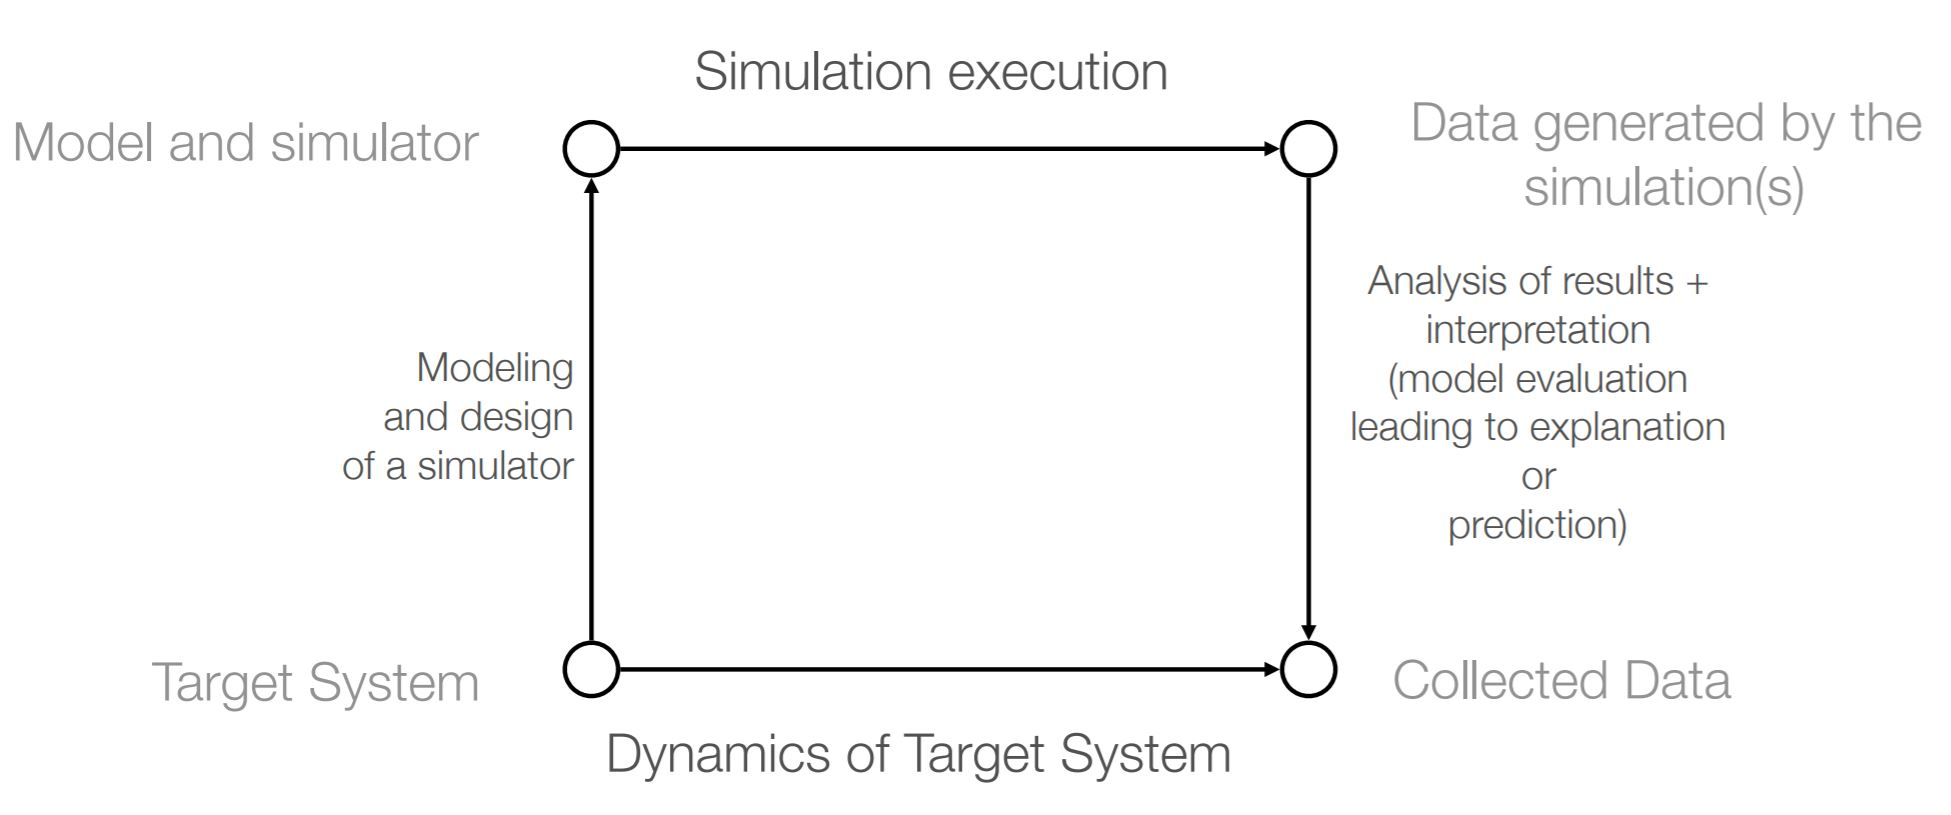
\includegraphics[width=0.9\textwidth,height=\textheight,keepaspectratio]{Figures/Vario/Simulazione.jpg}
\caption[Ciclo di vita di una simulazione]{Ciclo di vita di una simulazione}
\label{fig:Simulazione}
\end{figure}

\newpage

\subsection{Sistema multiagente}
Un sistema multiagente o (sistema ad agenti multipli) è un insieme di agenti situati in un certo ambiente ed interagenti tra loro mediante una opportuna organizzazione. Un agente è un'entità caratterizzata dal fatto di essere, almeno parzialmente, autonoma, sia essa un programma informatico, un robot, un essere umano, e così via.

\begin{figure}[ht]
\centering
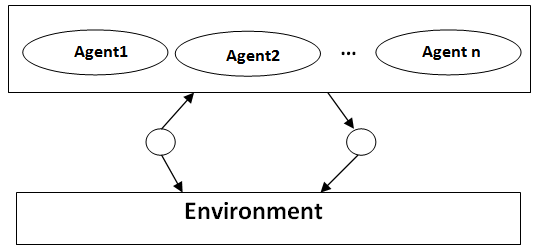
\includegraphics[width=0.9\textwidth,height=\textheight,keepaspectratio]{Figures/Vario/MAS.png}
\caption[Interazione di più agenti con l'ambiente]{Interazione di più agenti con l'ambiente}
\label{fig:MAS}
\end{figure}

\noindent Oggetto di ricerche da lunga data in intelligenza artificiale, i sistemi ad agenti multipli costituiscono un'interessante tipologia di modellazione di società, e hanno a questo riguardo vasti campi d'applicazione, che si estendono fino alle scienze umane e sociali (economia, sociologia, etc.). \cite{SistemaMultiagente}\\

\noindent Un sistema multiagente, per essere definito tale, deve rispettare le seguenti caratteristiche: \cite{CaratteristicheMAS}
\begin{itemize}
\item Autonomia: ogni agente deve essere almeno parzialmente indipendente.
\item Vista locale: nessun agente deve avere la vista globale del sistema.
\item Decentralizzazione: nessun agente può controllare l'intero sistema.
\end{itemize}

\newpage
\subsubsection{Modelli di interazione tra agenti}
Due o più agenti interagiscono tra loro se sono in una relazione dinamica attraverso sequenza di azioni reciproche. Due agenti sono portati ad interagire tra di loro quando non è possibile effettuare o portare a termine un determinato compito da parte di un agente singolo. Ciò può accadere a causa di risorse insufficienti, abilità insufficienti oppure per un approccio distribuito.\\

\noindent Esistono diversi modelli di interazione tra agenti, che possono essere suddivisi a loro volta in due grandi categorie: modelli di interazione diretta e modelli di interazione indiretta.

\begin{figure}[ht]
\centering
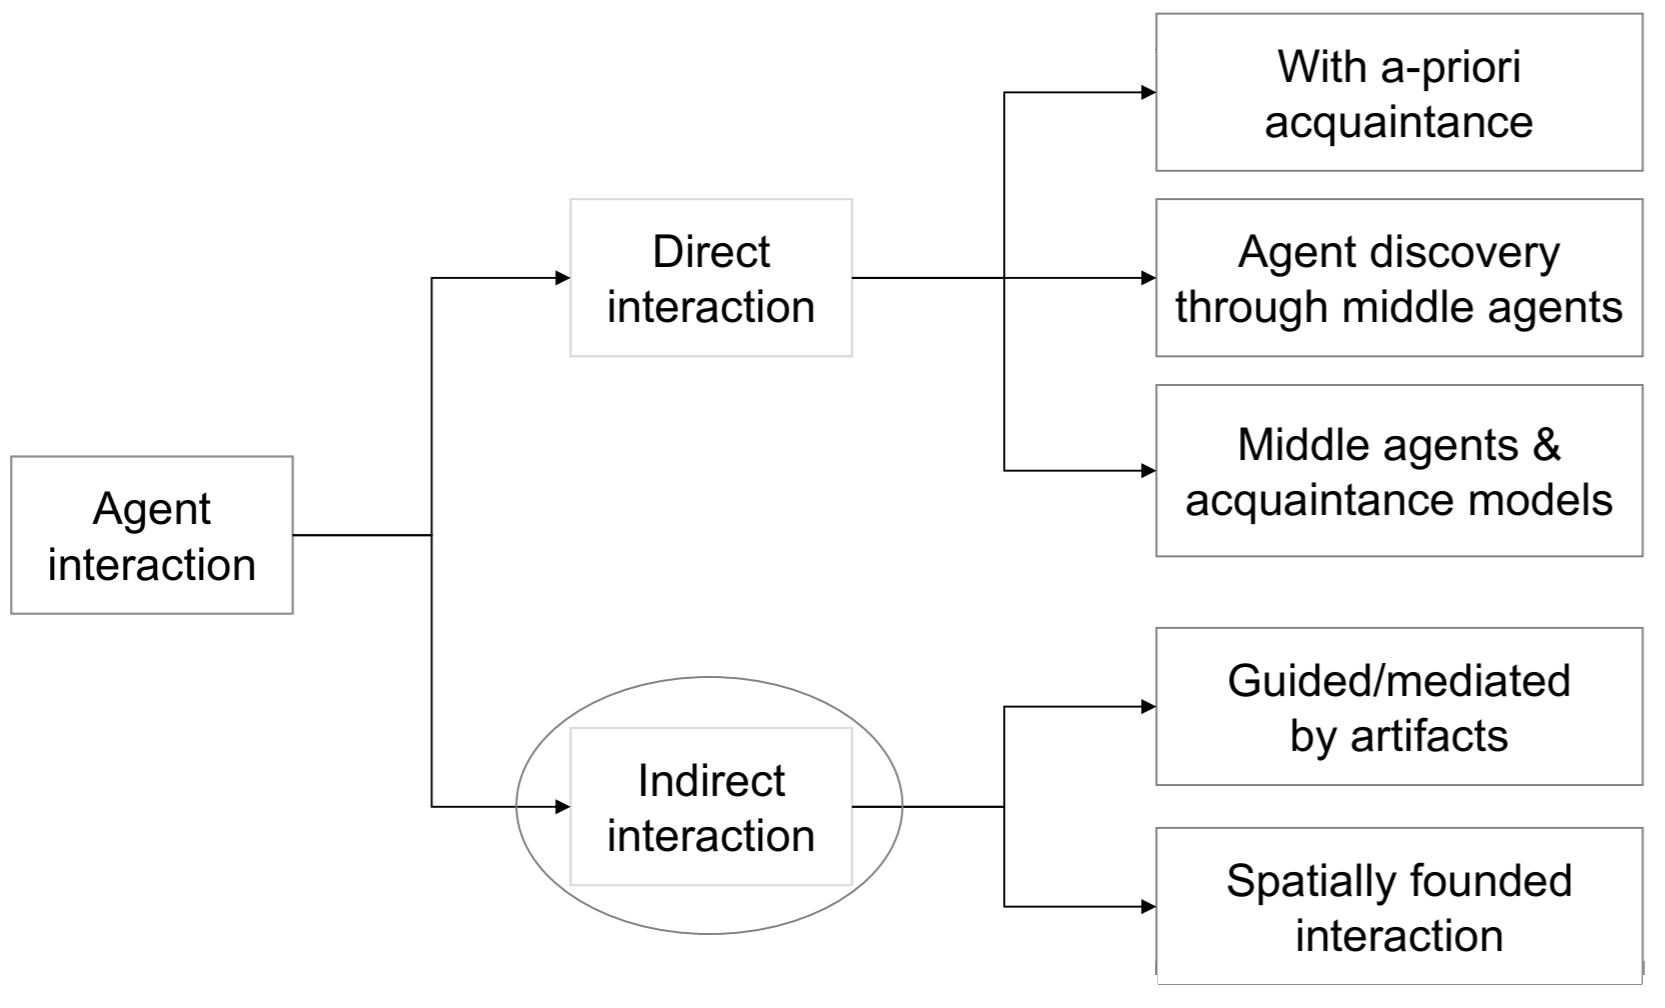
\includegraphics[width=\textwidth,height=\textheight,keepaspectratio]{Figures/Vario/Agent_Interaction.png}
\caption[Modelli di interazione tra agenti]{Modelli di interazione tra agenti}
\label{fig:Agent_Interaction}
\end{figure}

\noindent Nei modelli ad interazione diretta gli agenti sono in grado di comunicare direttamente tra di loro. Lo scambio di informazioni è reso possibile grazie all'utilizzo di un agent communication language (ACL) e di una struttura dei messaggi. La comunicazione tra due agenti di questo genere avviene quindi maniera indiscriminata dato che l'informazione va dal mittente al destinatario senza alcun tipo di dispersione e/o intermediario esterno. \\ Questi modelli sono facilmente implementabili e simili a sistemi distribuiti già esistenti, anche se allo stesso tempo sono presenti regole strette sul metodo di comunicazione e ogni agente deve essere a conoscenza di un altro agente prima di poterci comunicare.\\

\noindent Nei modelli ad interazione indiretta invece gli agenti interagiscono attraverso un ente che funziona di intermediario. Questo ente fornisce dei meccanismi di comunicazioni e delle regole dia accesso. L'implementazione di un modello del genere permette di avere un'interazione mediata, e quindi maggior possibilità di controllo, seppur l'implementazione risulta molto complessa per alcuni contesti e alcuni sistemi distribuiti.


\subsubsection{Tipologie di ambienti}
Esistono diverse tipologie di ambienti che possono essere caratterizzati nelle seguenti categorie:
\begin{table}[ht]
\centering
\resizebox{\textwidth}{!}{%
\begin{tabular}{lll}
\multicolumn{1}{c}{\cellcolor[HTML]{EFEFEF}\textbf{Accessible}}                                                                                                                                             &  & \multicolumn{1}{c}{\cellcolor[HTML]{EFEFEF}\textbf{Inaccessible}}                                                                                                                      \\
\begin{tabular}[c]{@{}l@{}}E' possibile conoscere tutte le informazioni \\ riguardanti le possibili combinazione \\ dell'evoluzione dell'ambiente.\end{tabular}                                             &  & \begin{tabular}[c]{@{}l@{}}Non è possibile conoscere tutte le informazioni \\ riguardanti le possibili combinazione \\ dell'evoluzione dell'ambiente.\end{tabular}                     \\
                                                                                                                                                                                                            &  &                                                                                                                                                                                        \\
\multicolumn{1}{c}{\cellcolor[HTML]{EFEFEF}\textbf{Deterministic}}                                                                                                                                          &  & \multicolumn{1}{c}{\cellcolor[HTML]{EFEFEF}\textbf{Non Deterministic}}                                                                                                                 \\
\begin{tabular}[c]{@{}l@{}}E' possibile conosce in maniera deterministica \\ tutti i cambiamenti che una certa azione \\ porta al sistema.\end{tabular}                                                     &  & \begin{tabular}[c]{@{}l@{}}Non è possibile conosce in maniera \\ deterministica tutti i cambiamenti che \\ una certa azione porta al  sistema.\end{tabular}                            \\
                                                                                                                                                                                                            &  &                                                                                                                                                                                        \\
\multicolumn{1}{c}{\cellcolor[HTML]{EFEFEF}\textbf{Episodic}}                                                                                                                                               &  & \multicolumn{1}{c}{\cellcolor[HTML]{EFEFEF}\textbf{Non Episodic}}                                                                                                                      \\
\begin{tabular}[c]{@{}l@{}}Le performance di un agente dipendono dal \\ numero di episodi discreti avvenuti,  con nessun\\ rapporto con le performance dell'agente \\ in uno scenario diverso.\end{tabular} &  & \begin{tabular}[c]{@{}l@{}}Le performance di un agente non dipendono \\ dal numero di episodi discreti avvenuti, \\ e l'agente prende decisioni su \\ scenari differenti.\end{tabular} \\
                                                                                                                                                                                                            &  &                                                                                                                                                                                        \\
\multicolumn{1}{c}{\cellcolor[HTML]{EFEFEF}\textbf{Static}}                                                                                                                                                 &  & \multicolumn{1}{c}{\cellcolor[HTML]{EFEFEF}\textbf{Dynamic}}                                                                                                                           \\
\begin{tabular}[c]{@{}l@{}}Non è soggetto a variazioni sul suo stato \\ durante il corso della finestra temporale\\ in cui l'agente sta agendo.\end{tabular}                                                &  & \begin{tabular}[c]{@{}l@{}}E' soggetto a variazioni sul suo stato \\ durante il corso della finestra temporale \\ in cui l'agente sta agendo.\end{tabular}                             \\
                                                                                                                                                                                                            &  &                                                                                                                                                                                        \\
\multicolumn{1}{c}{\cellcolor[HTML]{EFEFEF}\textbf{Discrete}}                                                                                                                                               &  & \multicolumn{1}{c}{\cellcolor[HTML]{EFEFEF}\textbf{Continuous}}                                                                                                                        \\
\begin{tabular}[c]{@{}l@{}}E' possibile rappresentare con una \\ cardinalità finita gli stati dell'ambiente.\end{tabular}                                                                                   &  & \begin{tabular}[c]{@{}l@{}}Non è possibile rappresentare con una \\ cardinalità finita gli stati dell'ambiente.\end{tabular}                                                          
\end{tabular}%
}
\caption{Diverse tipologie di ambiente}
\label{Ambiente}
\end{table}

\newpage

\subsection{Automated Guided Vehicle}
Un veicolo a guida autonoma (AGV) identifica dei veicoli, solitamente utilizzati in campo industriale per il trasporto di prodotti da un punto dello stabilimento ad un altro.\\

\begin{figure}[ht]
\centering
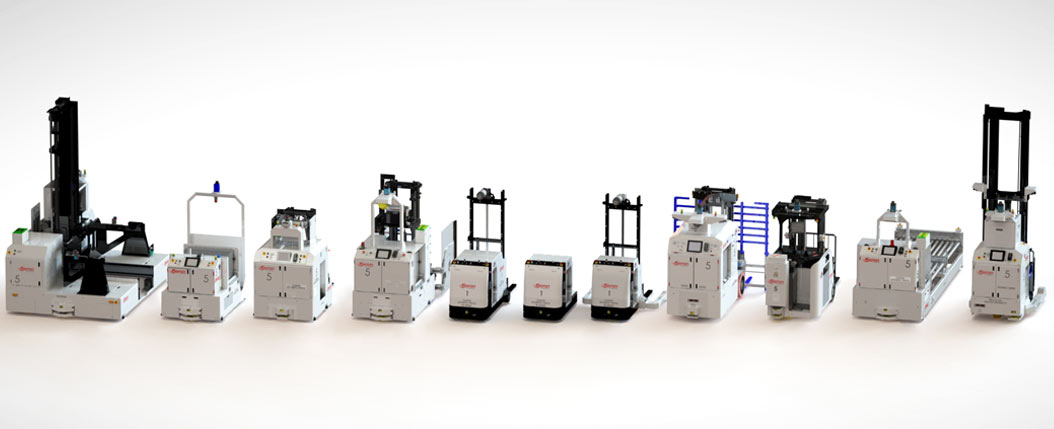
\includegraphics[width=\textwidth,height=\textheight,keepaspectratio]{Figures/Vario/AGV.jpg}
\caption[Diversi modelli di AGV]{Diversi modelli di AGV}
\label{fig:AGV}
\end{figure}


\noindent Esistono numerose tecnologie adottate per la realizzazione di AGV, ognuna con vantaggi e svantaggi; la scelta tecnica di realizzazione infatti è fortemente correlata al problema e all'ambiente che si sta considerando.  degli AGV:
\begin{table}[ht]
\centering
\resizebox{0.8\textwidth}{!}{%
\begin{tabular}{lll}
\multicolumn{1}{c}{\cellcolor[HTML]{EFEFEF}\textbf{Navigation}}                                                                                                                         &                               & \multicolumn{1}{c}{\cellcolor[HTML]{EFEFEF}\textbf{Path decision}}                                                        \\
\begin{tabular}[c]{@{}l@{}}- Wired\\ - Guide tape\\ - Laser target navigation\\ - Inertial navigation\\ - Natural features navigation \\ - Vision guidance\\ - Geoguidance\end{tabular} &                               & \begin{tabular}[c]{@{}l@{}}- Frequence select mode\\ - Path select mode\\ - Magnetic tape mode\end{tabular}               \\
                                                                                                                                                                                        &                               &                                                                                                                           \\
\multicolumn{1}{c}{\cellcolor[HTML]{EFEFEF}\textbf{Traffic control}}                                                                                                                    & \multicolumn{1}{c}{\textbf{}} & \multicolumn{1}{c}{\cellcolor[HTML]{EFEFEF}\textbf{Battery charging}}                                                     \\
\begin{tabular}[c]{@{}l@{}}- Zone control\\ - Collision avoidance\\ - Combination control\end{tabular}                                                                                  &                               & \begin{tabular}[c]{@{}l@{}}- Battery swap\\ - Automatic and opportunity charging \\ - Automatic battery swap\end{tabular}
\end{tabular}%
}
\caption{Diverse tipologie di tecnologie utilizzate per realizzazione AGV}
\label{AGVchars}
\end{table}


\newpage

\subsection{Automated Guided Vehicle System}
\noindent Un sistema automatizzato di veicoli a guida autonoma (AGVS) permette di gestire molteplici AGV al fine di raggiungere un obiettivo o di portare a termine un compito.

\noindent Questi sistemi sono stati introdotti nel 1950, e da allora si sono trovati sempre più contesti e applicazioni in cui forniscono un'elevata utilità pratica. Essi permettono una gestione estremamente flessibile soprattutto in ambienti dinamici, dove le necessità continuano a variare nel tempo. Negli ultimi anni l'avvento di tecnologie sempre più avanzate e di MAS sempre più sofisticati ha portato ad un incremento delle performance di questi sistemi.


\subsubsection{Classificazione di un AGVS}
Un AGVS deve essere progettato e implementato considerando il contesto in cui ci si trova e le priorità che si presentano. Tutto sommato, un AGVS può essere classificato in base ai tre seguenti requisiti:
\begin{itemize}
\item \textbf{Percorso di guida:} Può essere statico, in cui la navigazione avviene seguendo una serie di percorsi prestabiliti (unidirezionale o bidirezionale) oppure può essere dinamico, in cui la navigazione dei veicoli avviene in maniera completamente autonoma.

\item \textbf{Capacità del veicolo:} Un AGV può avere una capacità di carico diversa da un altro, come ad esempio carico unitario e carico multiplo.

\item \textbf{Indirizzamento dei veicoli:} L'indirizzamento dei veicoli può essere indiretto, in cui un AGV può visitare solamente determinate stazioni, oppure diretto, in cui ogni AGV può visitare ogni stazione.

\end{itemize}

\subsubsection{Performance di un AGVS}
Solitamente la valutazione delle performance di un AGVS avviene tramite simulazione che, attraverso la raccolta di parametri rilevanti, permette di misurare le performance di un sistema rispetto ad un altro. Esempi di parametri di produzione che possono essere valutati di un AGVS sono:
\begin{itemize}
\setlength\itemsep{0.1em}
    \item Ordini svolti
    \item Tempo medio di attesa per ordini pronti
    \item Numero di conflitti
\end{itemize}

\subsection{Lavori precedenti}
Nonostante esistano parecchi lavori e pubblicazioni che riguardano AGV e AGVS, non è stato semplice trovare indicazioni che potessero guidare le scelte implementative a causa della scarsità di simulazioni che riguardano questi argomenti.\\

\noindent Nonostante ciò, due lavori sono stati molto utili:  ”Evaluation of automatic guided vehicle systems” \cite{EvaluationAGVS}, che ci ha permesso di individuare e definire le metriche utili alla valutazione del nostro simulatore e "Multi Agent Simulation for Decision Making in Warehouse Management” 1\cite{MAS_Warehouse}, in cui si analizza e simula un sistema complesso in un ambiente molto simile al nostro caso di studio.
Molte delle scelte non arbitrarie del progetto, quindi, sono prese o ricavate dai due documenti sopra citati.

\newpage
%%%%%%%%%%%%%%%%%%%%%%%%%%%%%%%%%%%%%%%%%%%%%%%
% Descrizione del dominio
%%%%%%%%%%%%%%%%%%%%%%%%%%%%%%%%%%%%%%%%%%%%%%%
\section{Descrizione del dominio}
\subsection{Azienda}
LDE s.r.l nasce nel 1997 come azienda per il trasporto e la logistica specializzata in abiti e tessuti. Ad oggi conta circa 30 dipendenti e un fatturato di oltre un milione di euro.

\subsection{Tipologia di lavoro e di ordini}
Il lavoro svolto da questa azienda consiste principalmente nell'elaborazione, preparazione, ricezione e spedizione di articoli. Gli articoli in questione possono essere di svariati tipi, dai vestiti agli accessori, da macchinari a utensili da cucina,..
In questo studio si andrà a considerare la parte del magazzino che tratta gli ordini inerenti agli articoli in ambito vestiario da loro trattati.

\subsection{Ambiente}
L'ambiente del magazzino preso da noi in considerazione consta di una zona per gli uffici (in basso a sinistra), 4 gate per caricare i camion (di cui uno chiuso, motivo per cui ne sono stati rappresentati tre sulla mappa della simulazione) e 8 corsie in cui sono posizionate le merci. Nella simulazione, tutto è rappresentato in scala 1:1 con piccole approssimazioni che non influiscono né sulle performance, né sull'aderenza alla realtà della simulazione.
Per quanto riguarda l'ambiente, le uniche assunzione che sono state fatte riguardano gli oggetti e, in particolare:
\begin{itemize}
    \item Gli oggetti nel magazzino sono sempre disponibili per un AGV che li richiede.
    \item Un AGV prende un oggetto posizionandosi in un punto preciso per la ricezione di quell’oggetto che viene posizionato sull’AGV da un ipotetico braccio meccanico.
\end{itemize}

\noindent Di seguito è riportata la cartina rappresentante la perimetria del dominio in questione, che verrà utilizzata nella fasi successive per ottenere un ambiente di simulazione verosimile a quello reale.

\begin{figure}
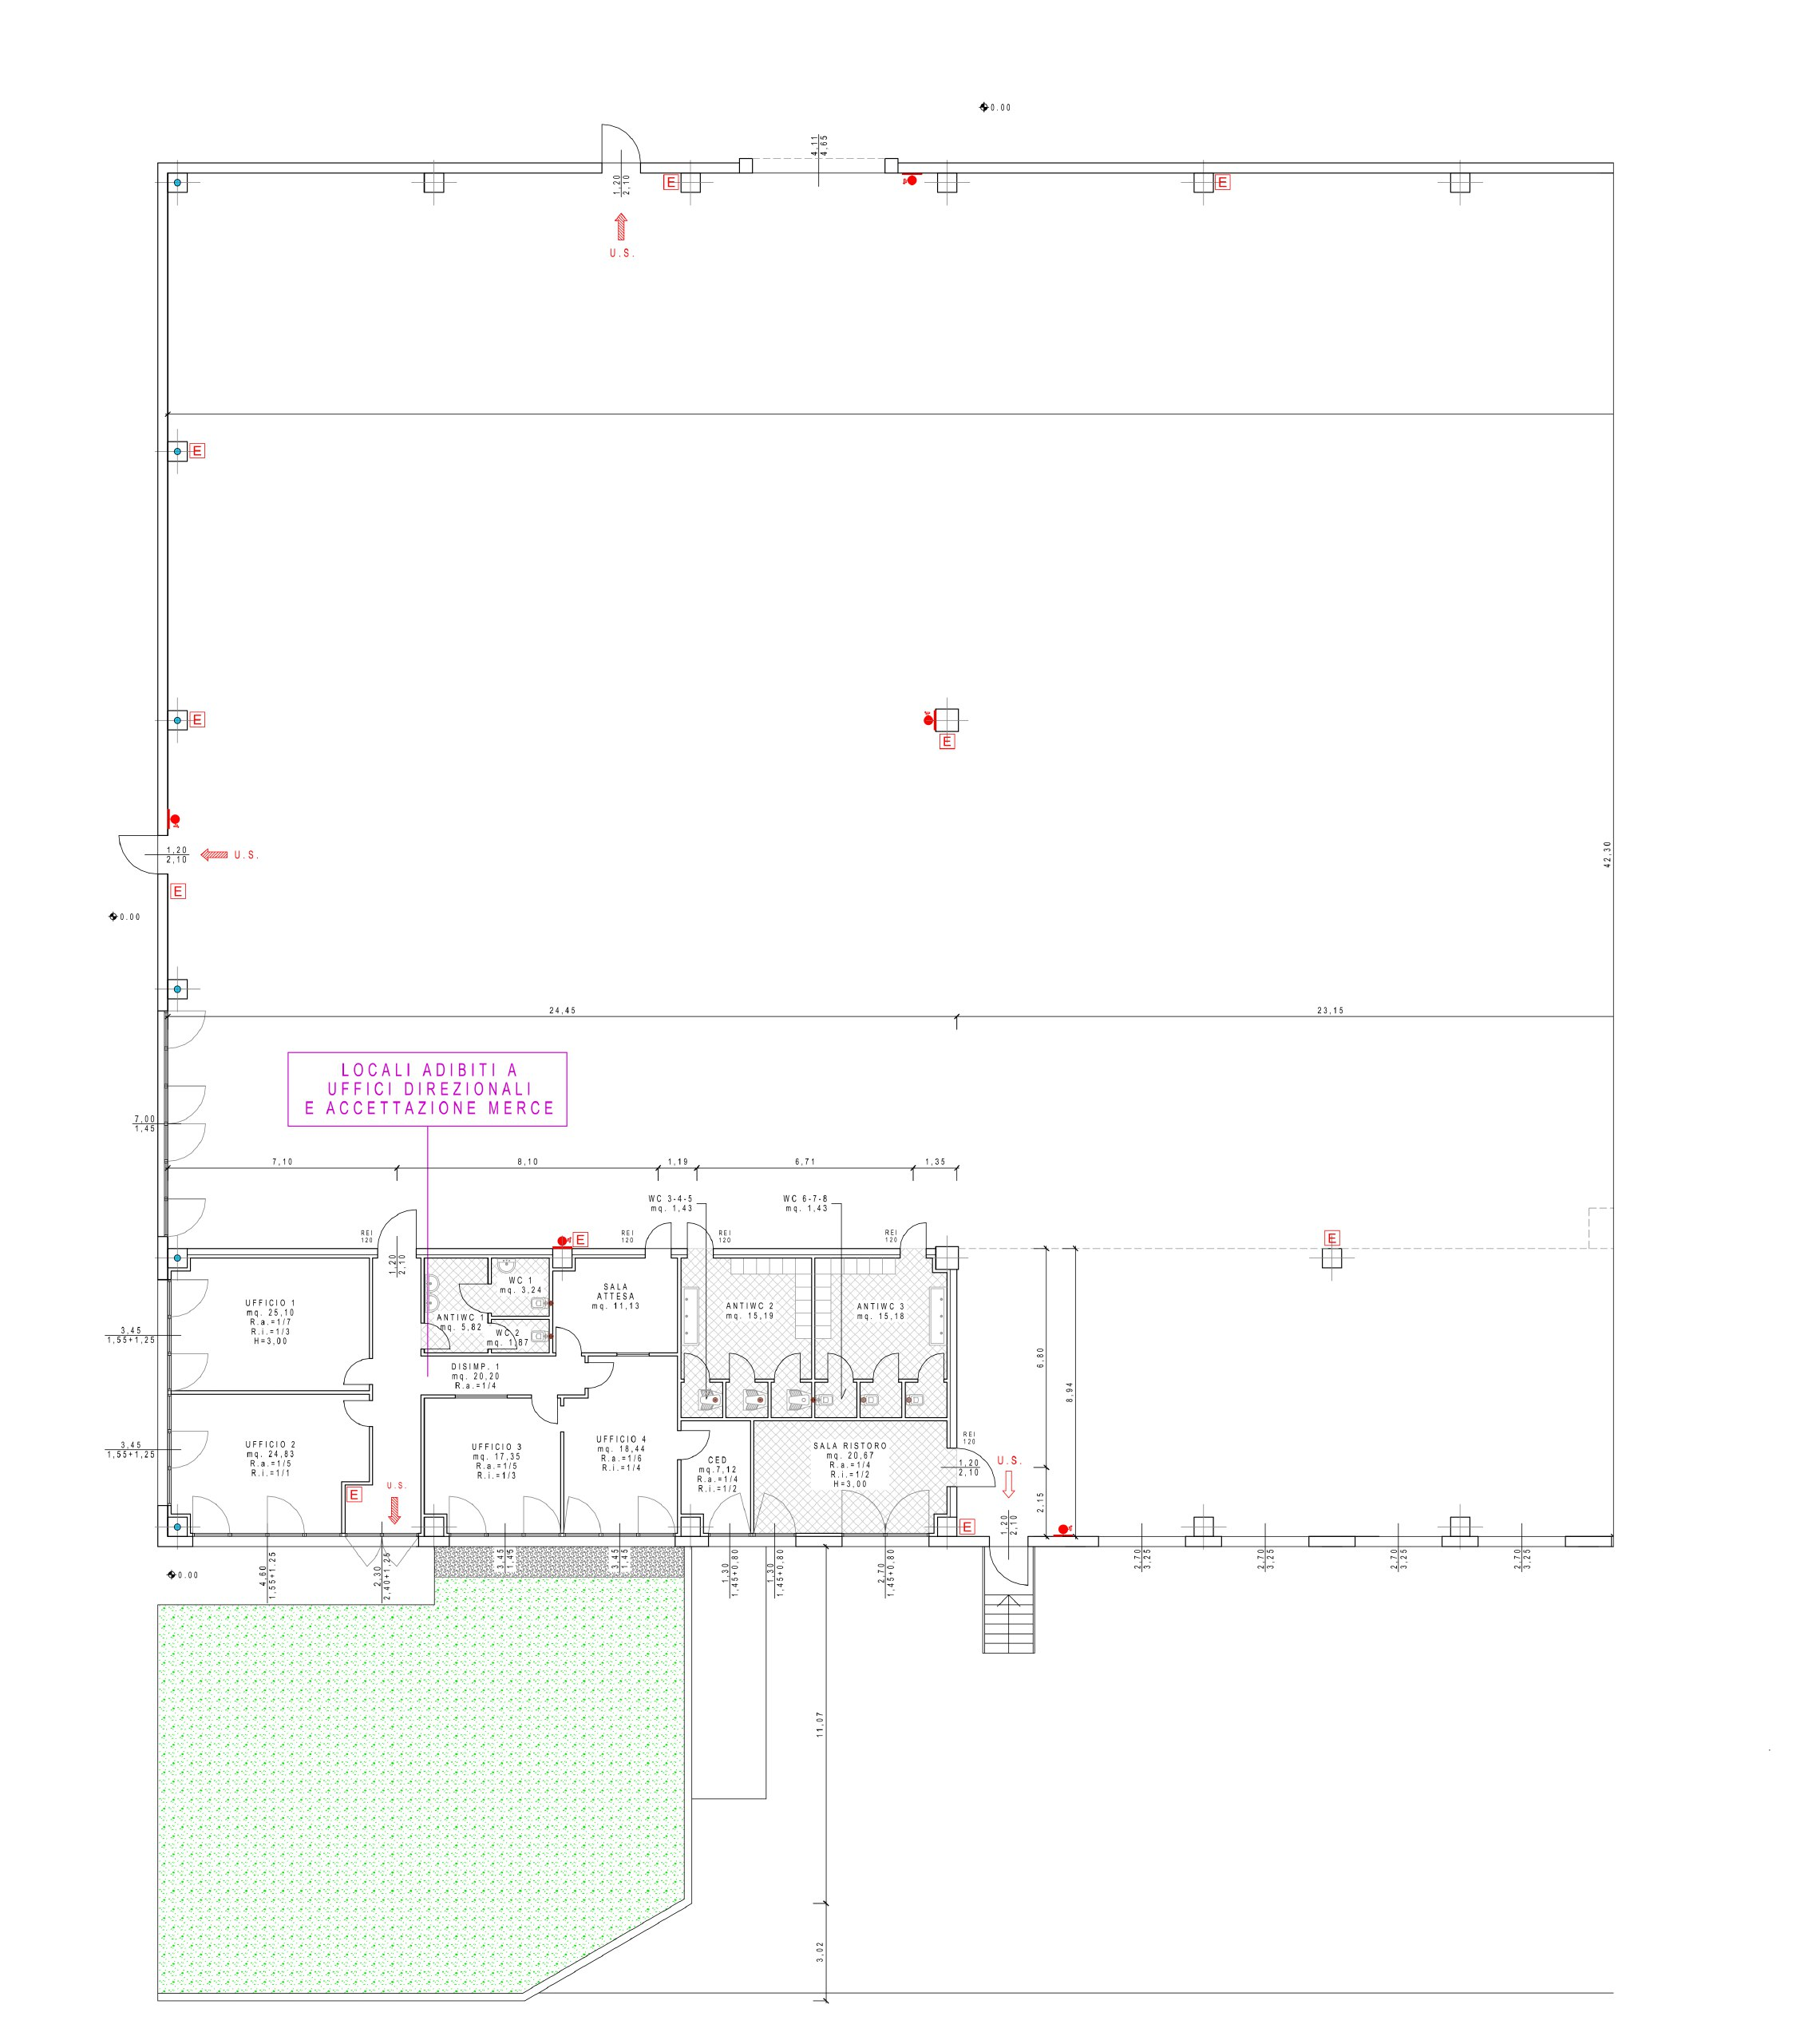
\includegraphics[width=\textwidth,height=\textheight,keepaspectratio]{Figures/Graphics/Zoom_Map.jpg}
\caption[Mappa fisica del magazzino]{Mappa fisica del magazzino}
\label{fig:Mappa_magazzino}
\end{figure}


\subsection{Lista degli ordini}
Insieme alla cartina del magazzino è stato possibile reperire un elenco di ordini che vengono svolti quotidianamente; la lista di cui si sta parlando contiene 2023 ordini differenti. Ciascun ordine contiene una lista di articoli che può variare e un unico destinatario, che può essere:
\begin{itemize}
\item Milano (MI)
\item Firenze (FI)
\item Como (CO)
\end{itemize}
Il seguente grafico riporta il numero di ordini presenti all'interno della lista per ciascuna destinazione.

\begin{figure}[ht]
\centering
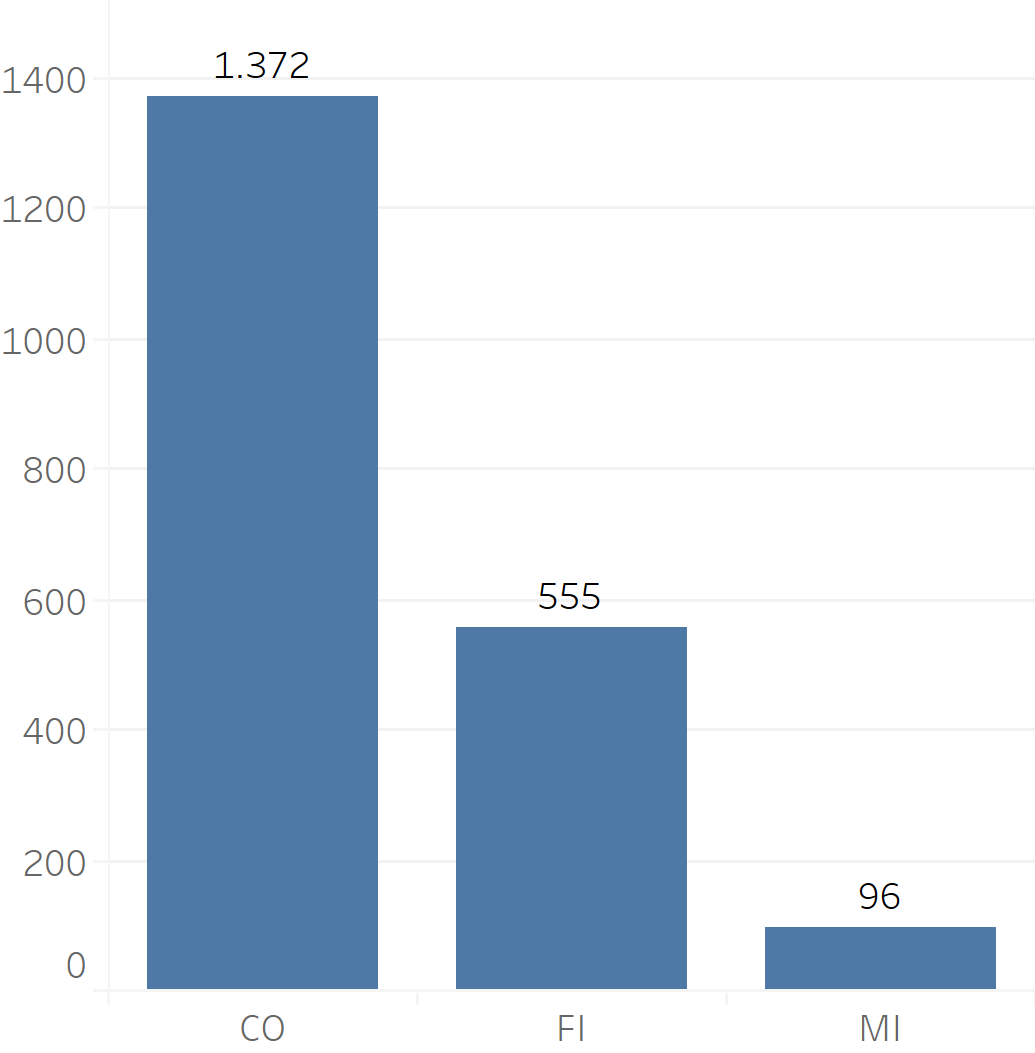
\includegraphics[width=0.7\textwidth,height=\textheight,keepaspectratio]{Figures/Initial_Dataset/Orders_client.png}
\caption[Numero di ordini per ciascun cliente]{Numero di ordini per ciascun cliente}
\label{fig:OrdiniClientiIniziali}
\end{figure}


\newpage
%%%%%%%%%%%%%%%%%%%%%%%%%%%%%%%%%%%%%%%%%%%%%%%
% Modellazione del problema
%%%%%%%%%%%%%%%%%%%%%%%%%%%%%%%%%%%%%%%%%%%%%%%
\section{Descrizione del modello}

\subsection{Ambiente del simulatore}
Una volta ottenuta la mappa del magazzino, si è andati a cercare di rappresentare la struttura del magazzino in maniera tale da renderla utilizzabile per un sistema di simulazione.
\begin{figure}[ht]
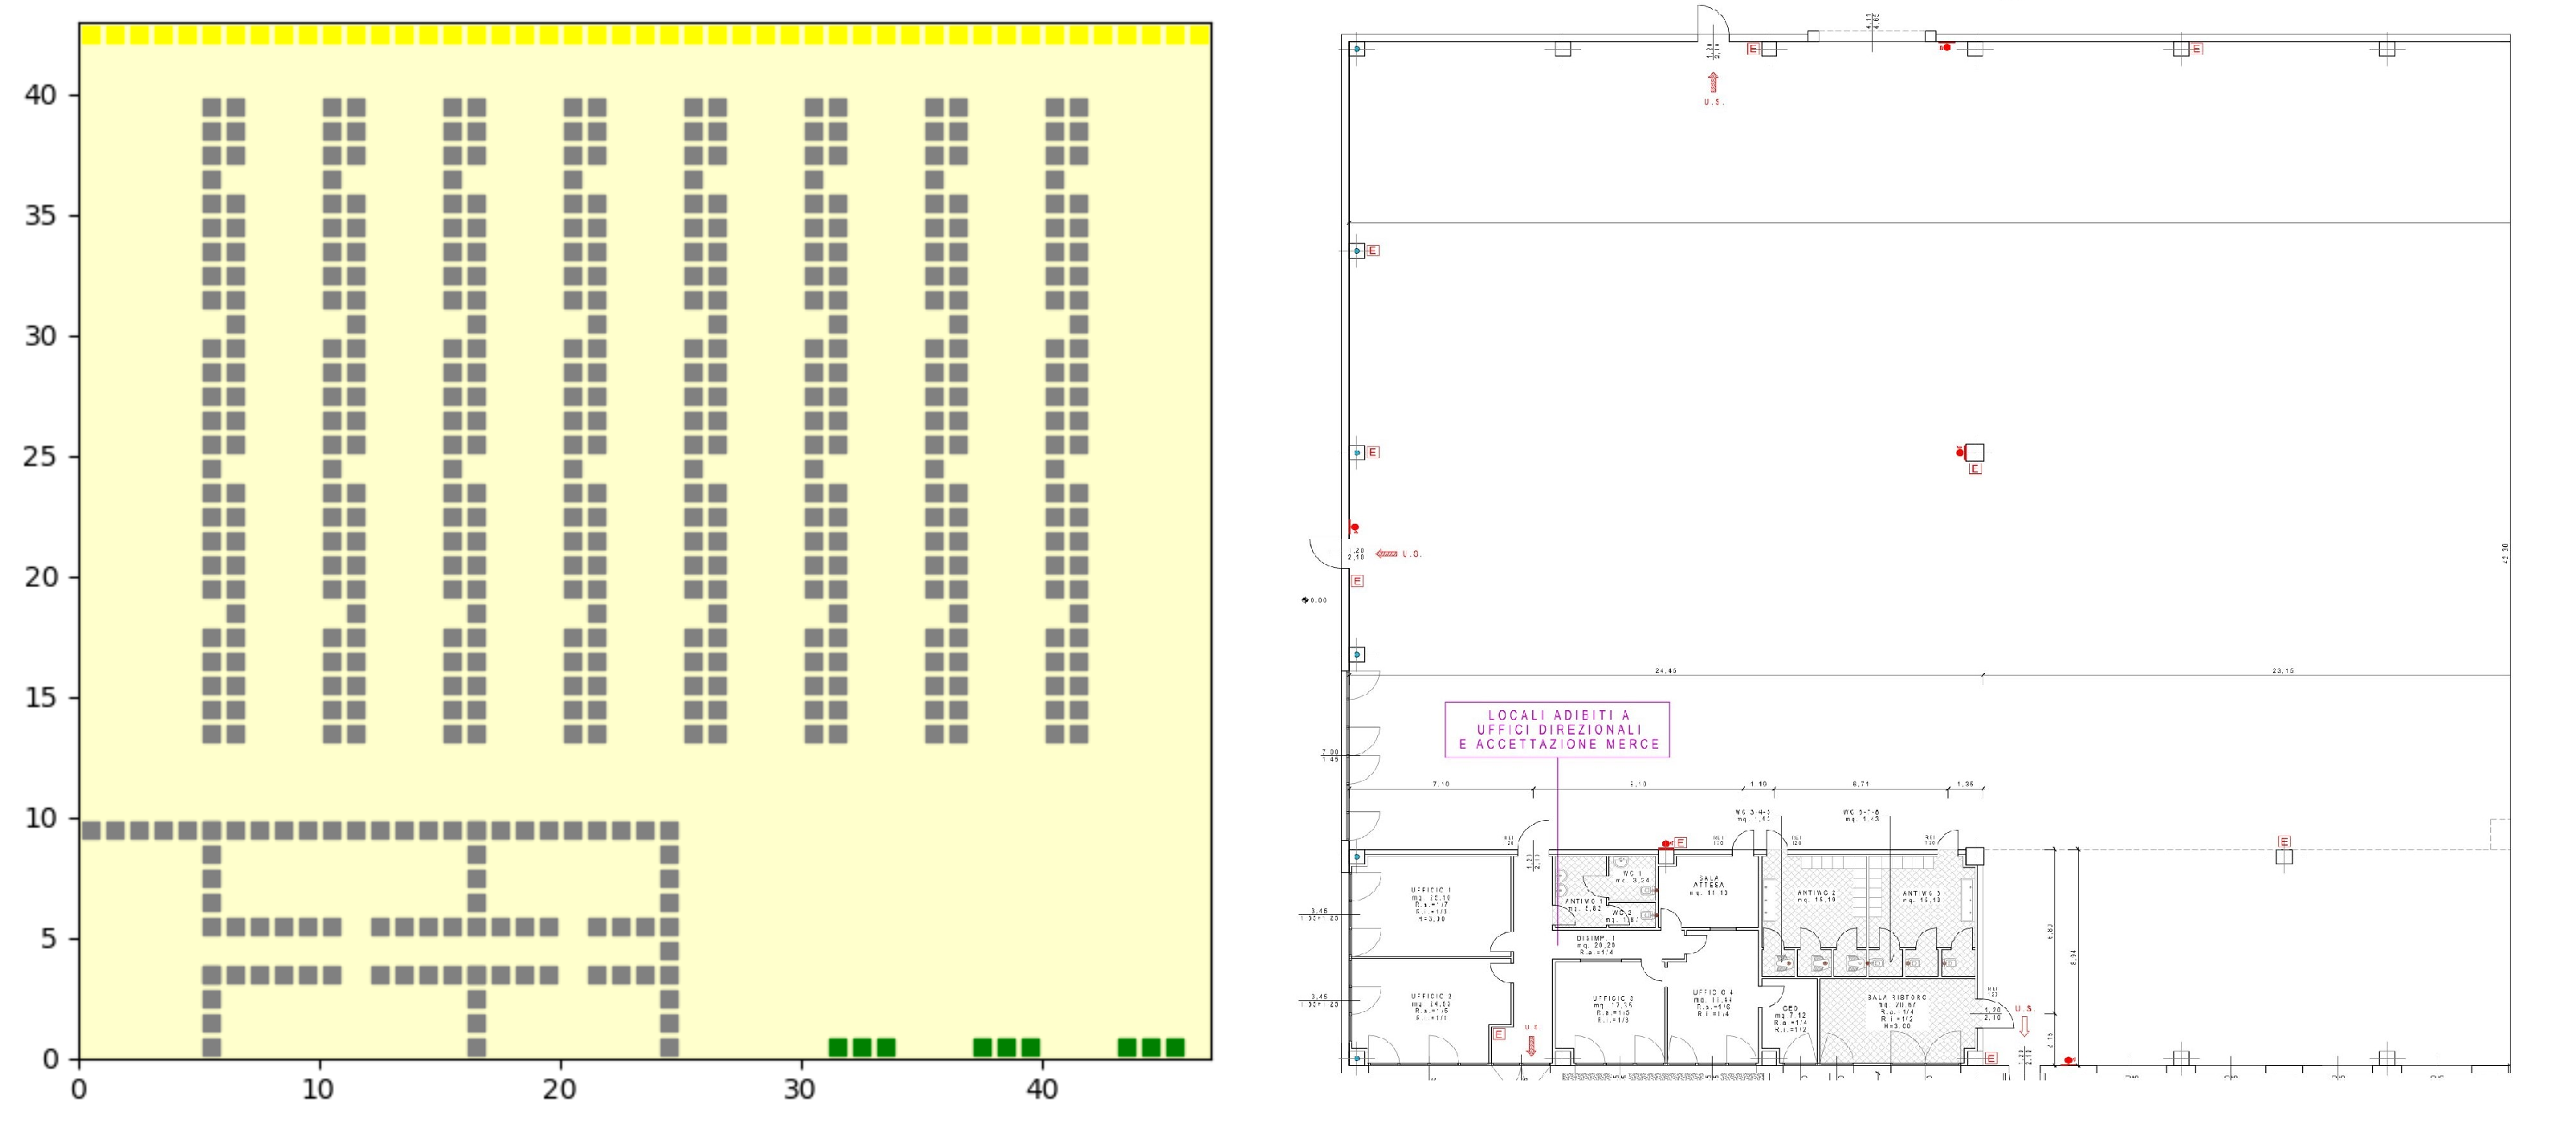
\includegraphics[width=\linewidth]{Figures/Graphics/Simulation_Domain.PNG}
\caption{Rappresentazione della mappa del magazzino sul simulatore}\label{fig:Rappresentazione_mappa}
\end{figure}

\noindent All'interno dell'ambiente sono stati definiti i seguenti elementi, di cui i primi 4 sono quelli fondamentali alla simulazione del problema e meglio descritti nella pagina seguente:

\begin{itemize}
\item Scaffalature
\item Punti di carico
\item Punti di scarico
\item Area di attesa
\item Area di ricarica
\item Uffici
\end{itemize}
\newpage


\begin{minipage}[ht]{0.45\linewidth}
\label{ambienteSimulatore}
\centering
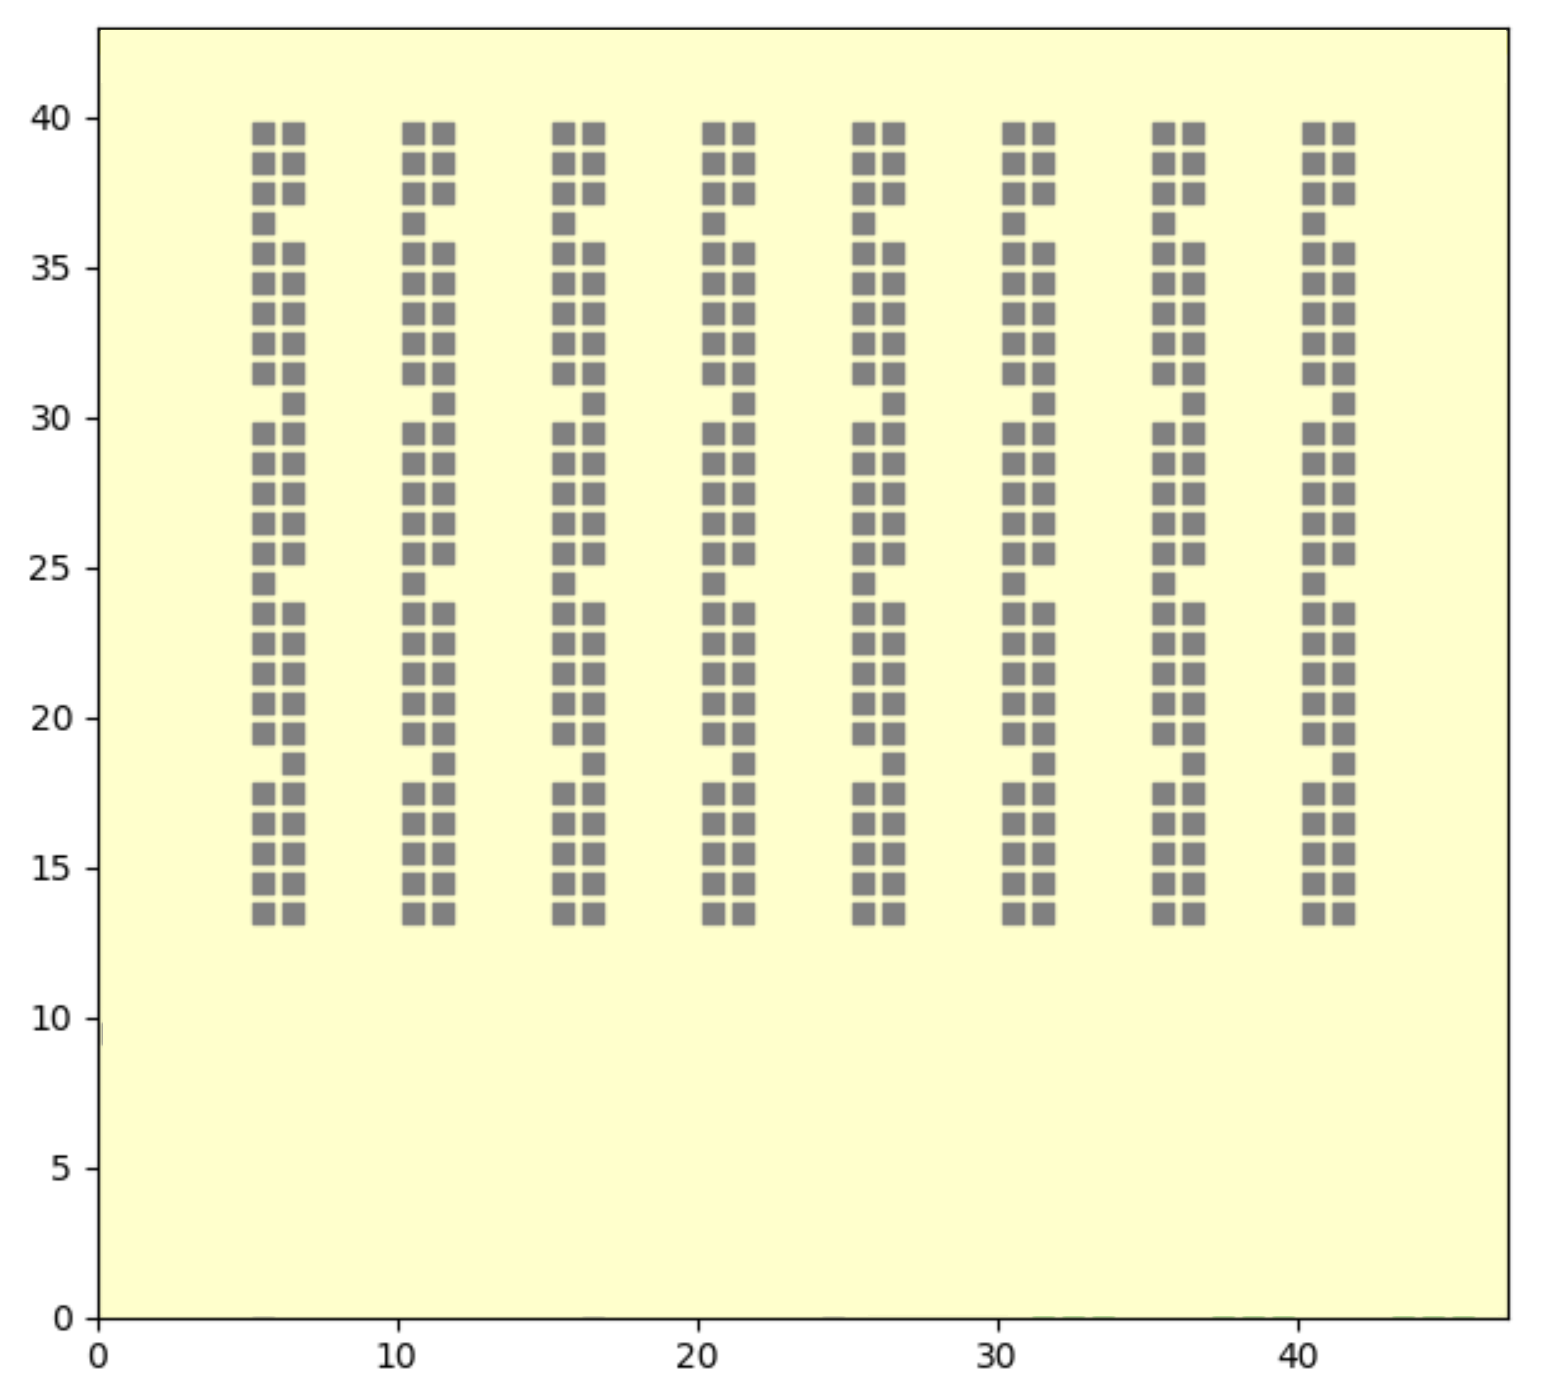
\includegraphics[width=\textwidth]{Figures/Map/Corsie.png}
\end{minipage}
\hspace{0.5cm}
\begin{minipage}[ht]{0.45\linewidth}
\centering
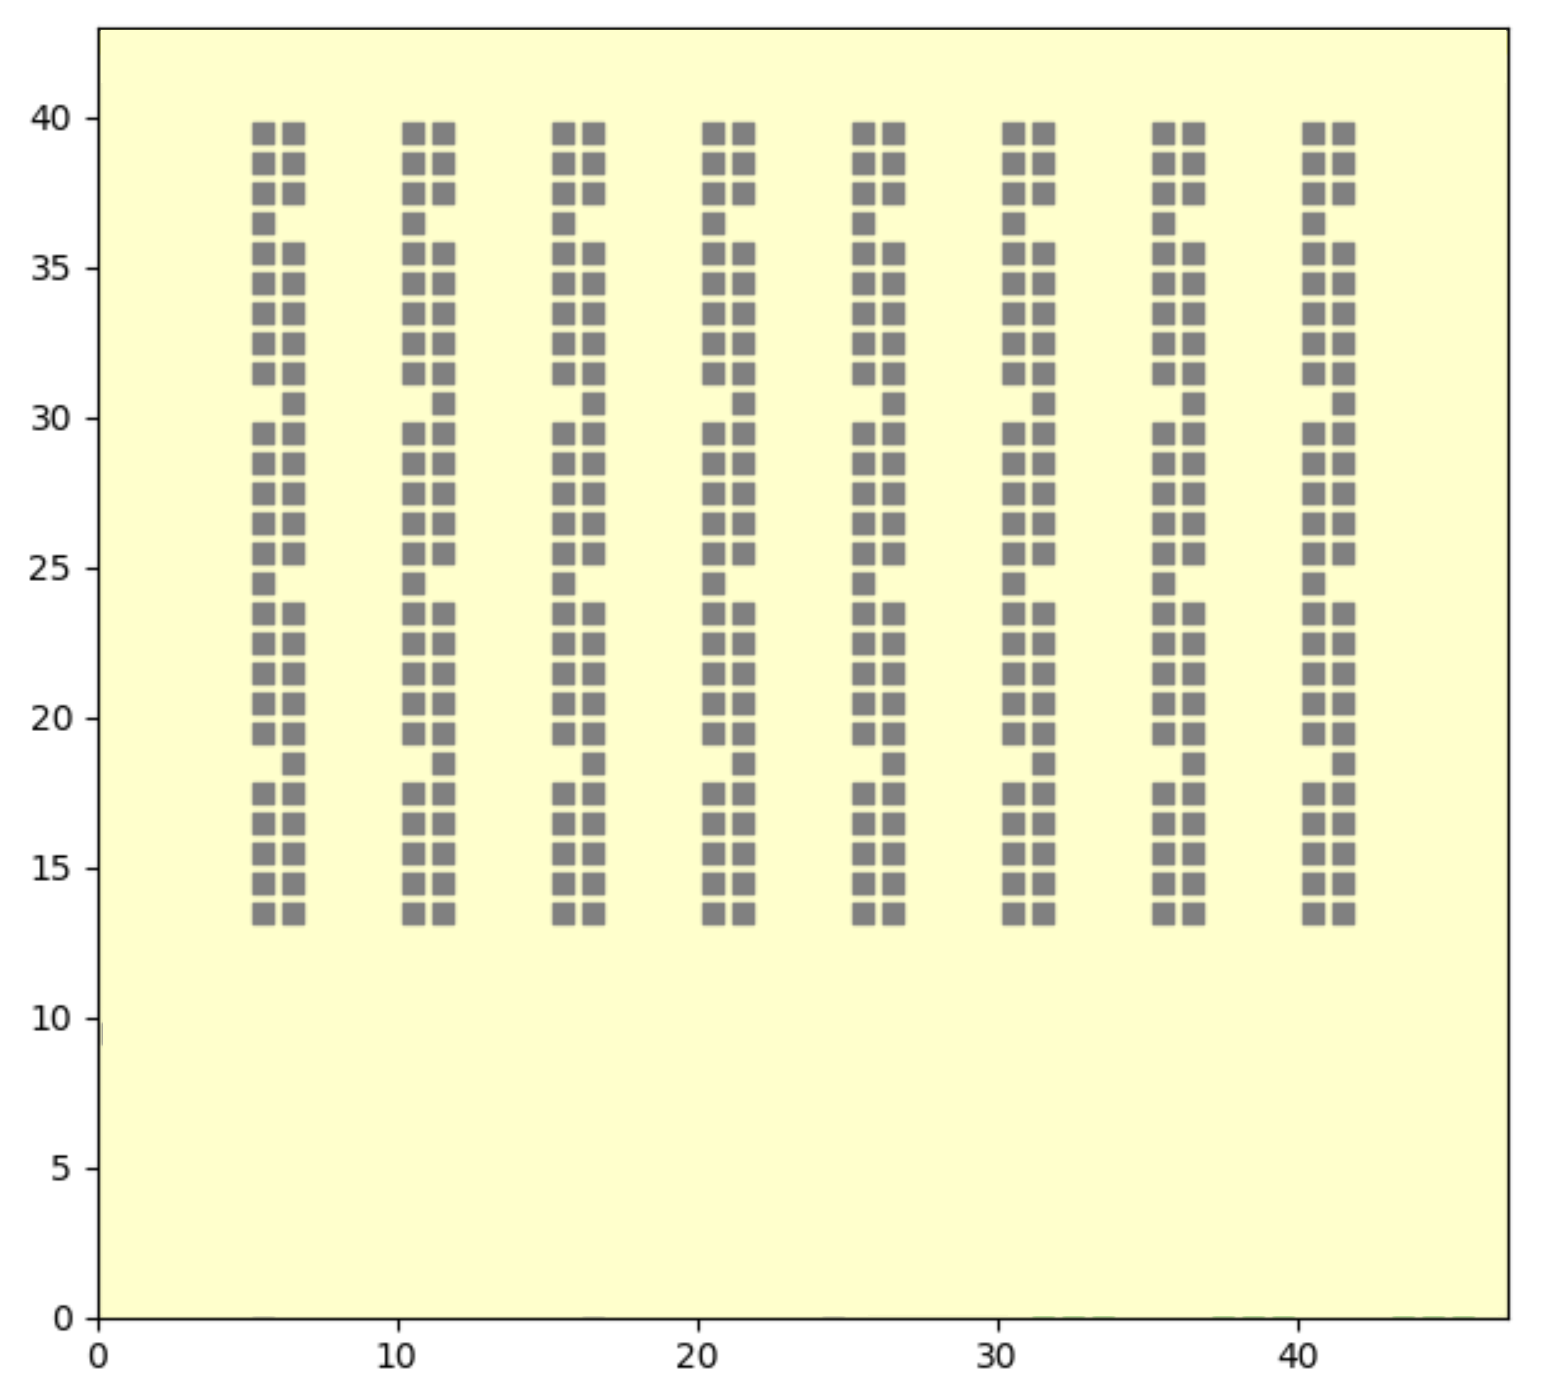
\includegraphics[width=\textwidth]{Figures/Map/Corsie.png}
\end{minipage}

\begin{minipage}[ht]{0.45\linewidth}
\vspace{0.2cm}
\textbf{Scaffalature:} Rappresentate con il colore grigio al centro dell'ambiente di simulazione, rispecchiando le corrispettive 8 scaffalature presenti all'interno del magazzino fisico.
\end{minipage}
\hspace{0.5cm}
\begin{minipage}[ht]{0.45\linewidth}
\vspace{0.2cm}
\textbf{Punti di carico:} Rappresentati con delle interruzioni della corsia sono collocati lungo le corsie stesse, dove l'AGV potrà accedere per poter prelevare le merci richieste.
\end{minipage}

\vspace{1cm}
\begin{minipage}[ht]{0.45\linewidth}
\centering
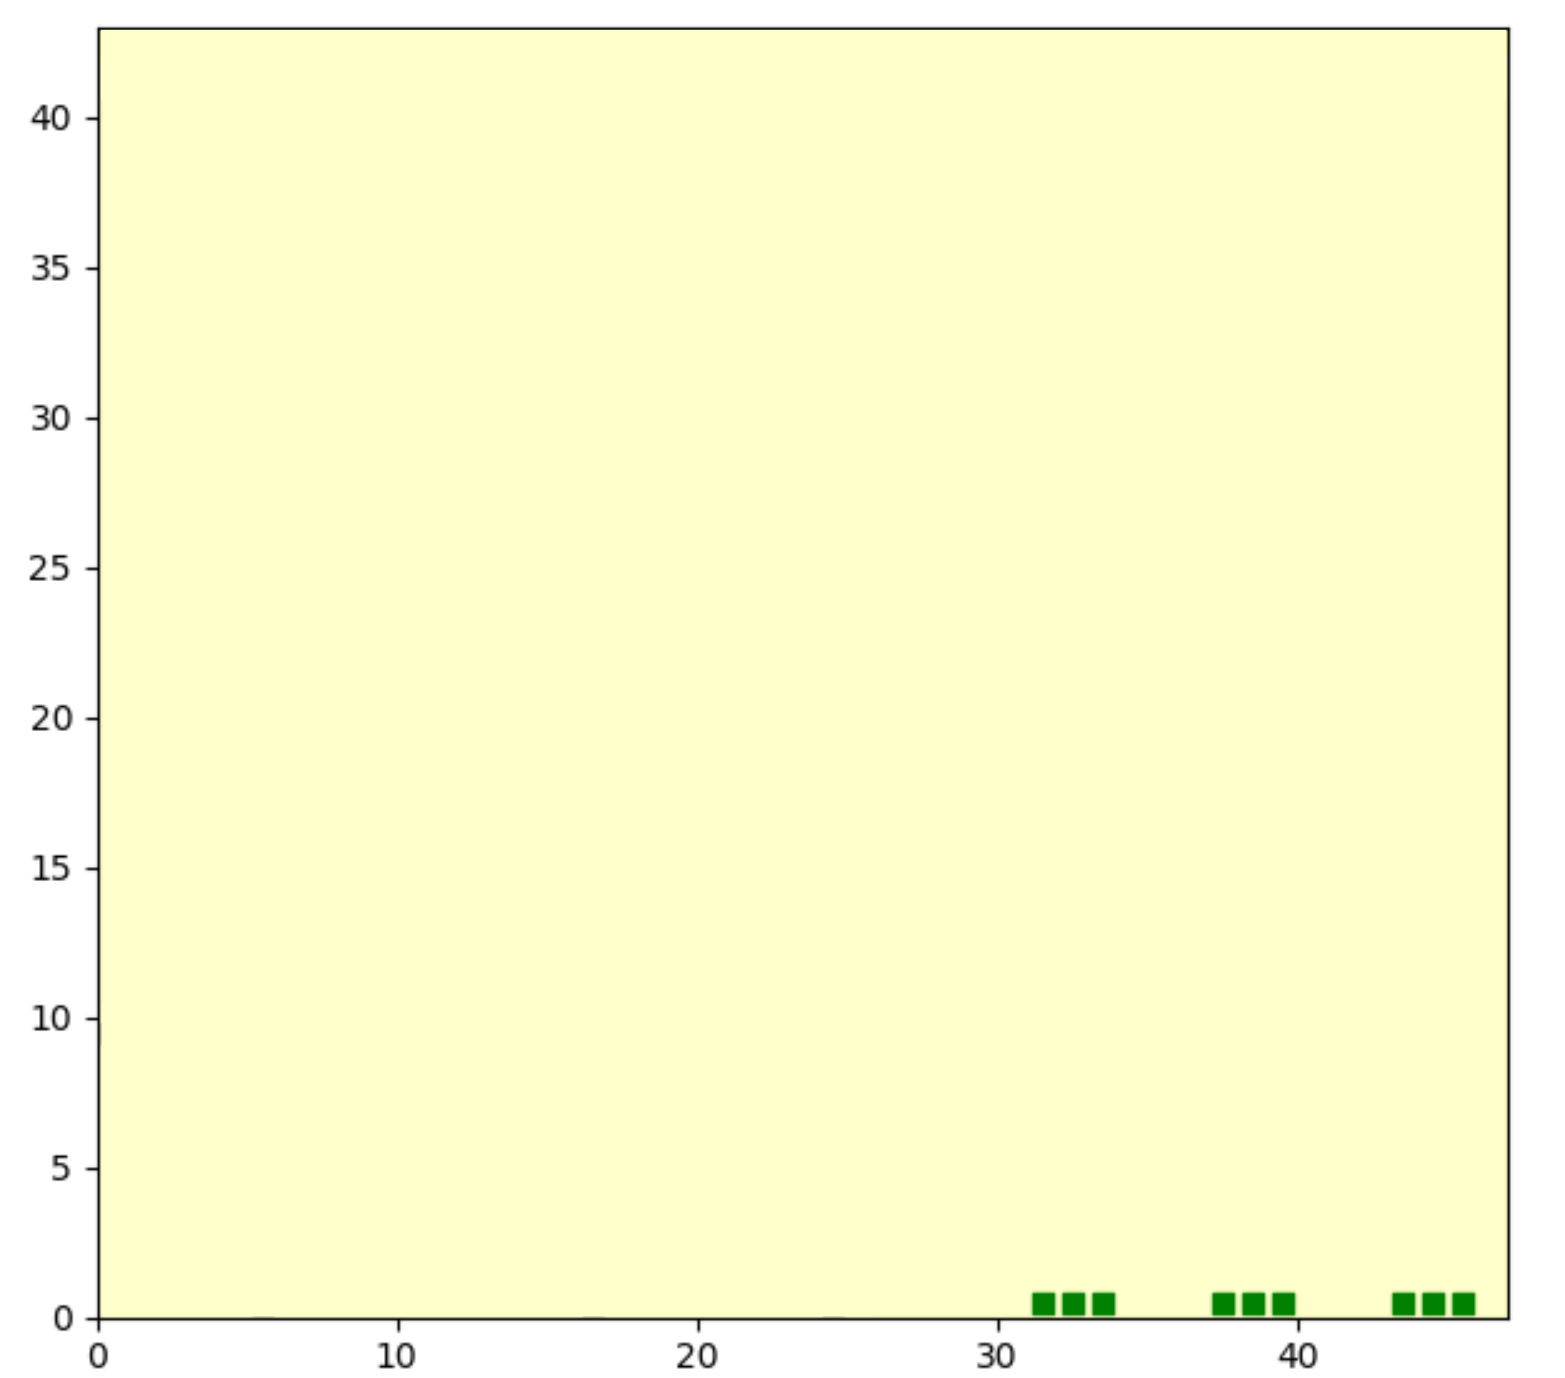
\includegraphics[width=\textwidth]{Figures/Map/Gates.png}
\end{minipage}
\hspace{0.5cm}
\begin{minipage}[ht]{0.45\linewidth}
\centering
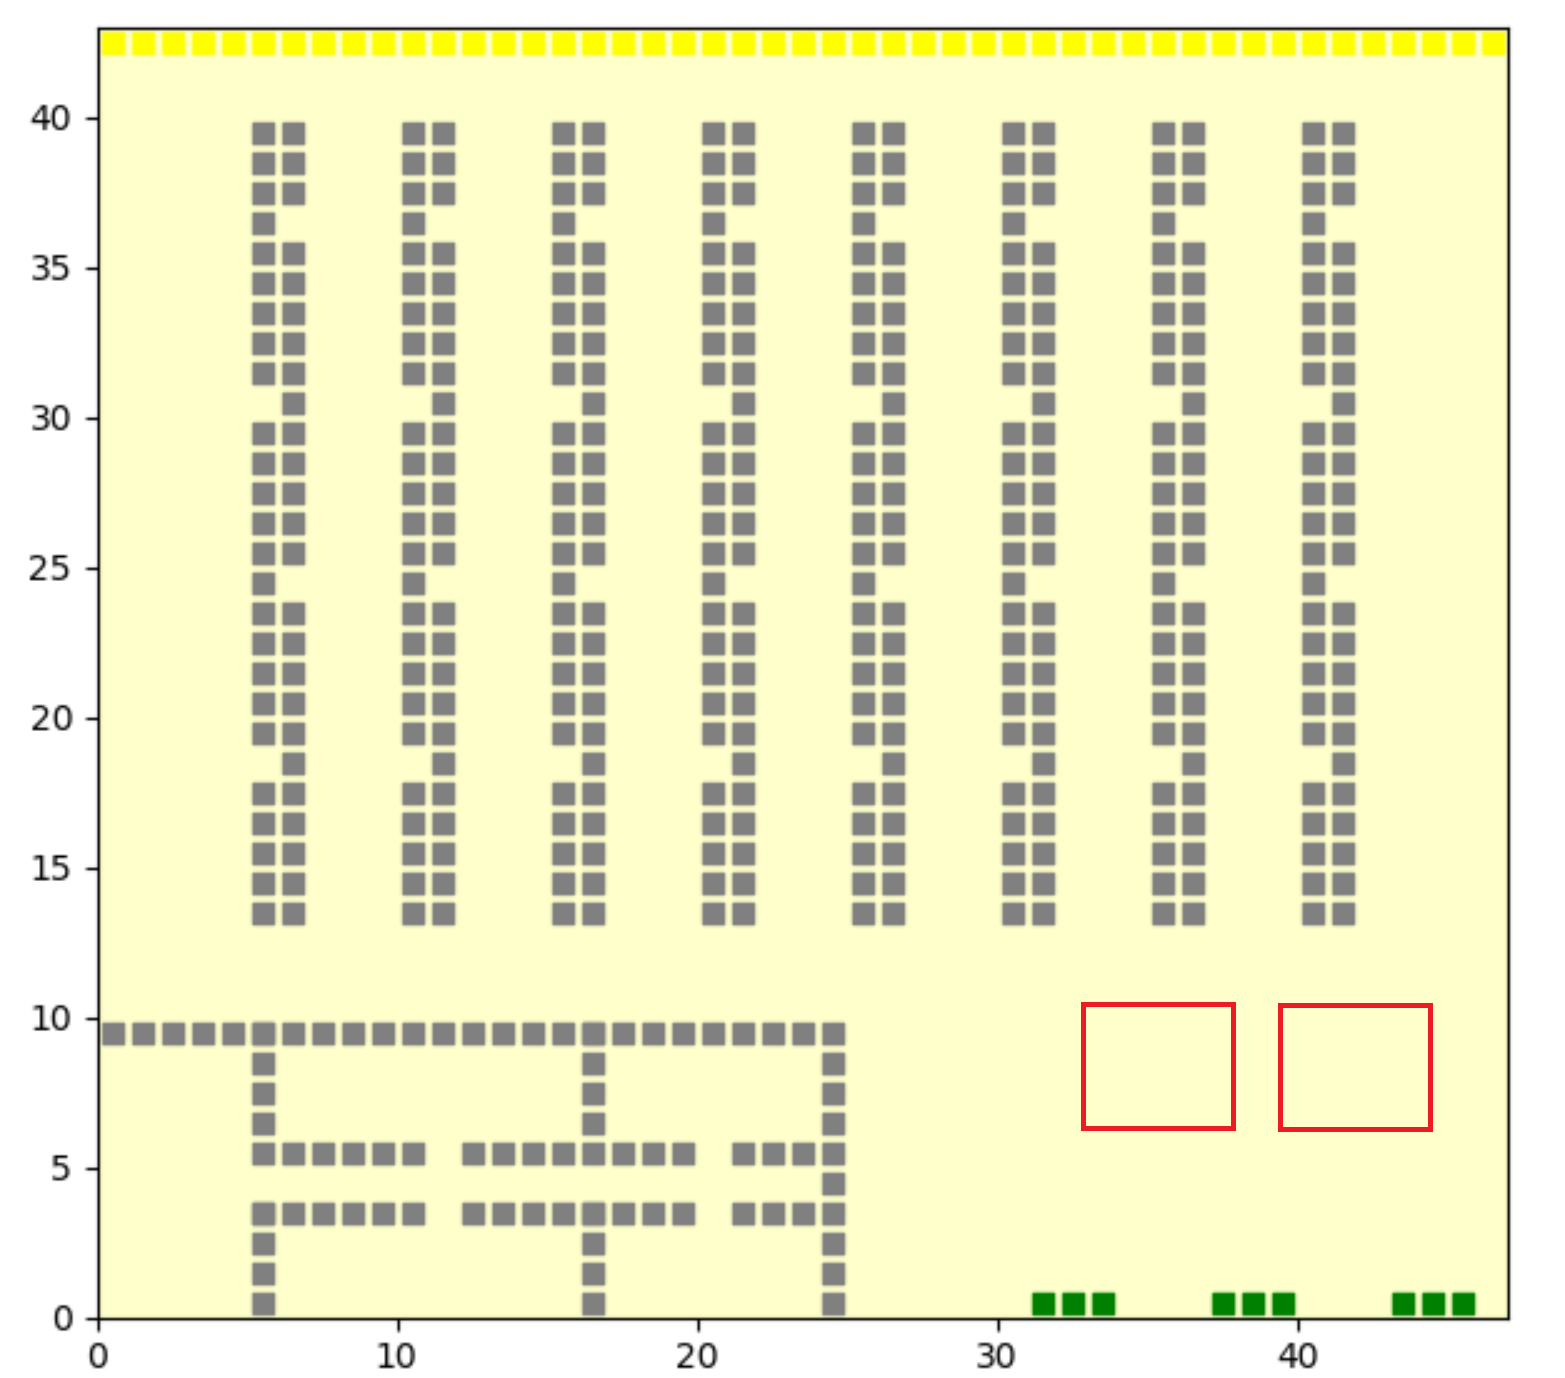
\includegraphics[width=\textwidth]{Figures/Map/WaitingArea.png}
\end{minipage}

\begin{minipage}[ht]{0.45\linewidth}
\vspace{0.2cm}
\textbf{Punti di scarico:} Rappresentati con il colore verde. Questi sono i punti in cui verranno rilasciate le merci prelevate dagli AGV in precedenza.
\end{minipage}
\hspace{0.5cm}
\begin{minipage}[]{0.45\linewidth}
\vspace{0.2cm}
\textbf{Area di attesa:} Indicata (nell'immagine) con due rettangoli rossi di fronte ai punti di scarico. Gli AGV in attesa di scaricare attenderanno qui il loro turno.
\end{minipage}

\begin{minipage}[ht]{0.45\linewidth}
\centering
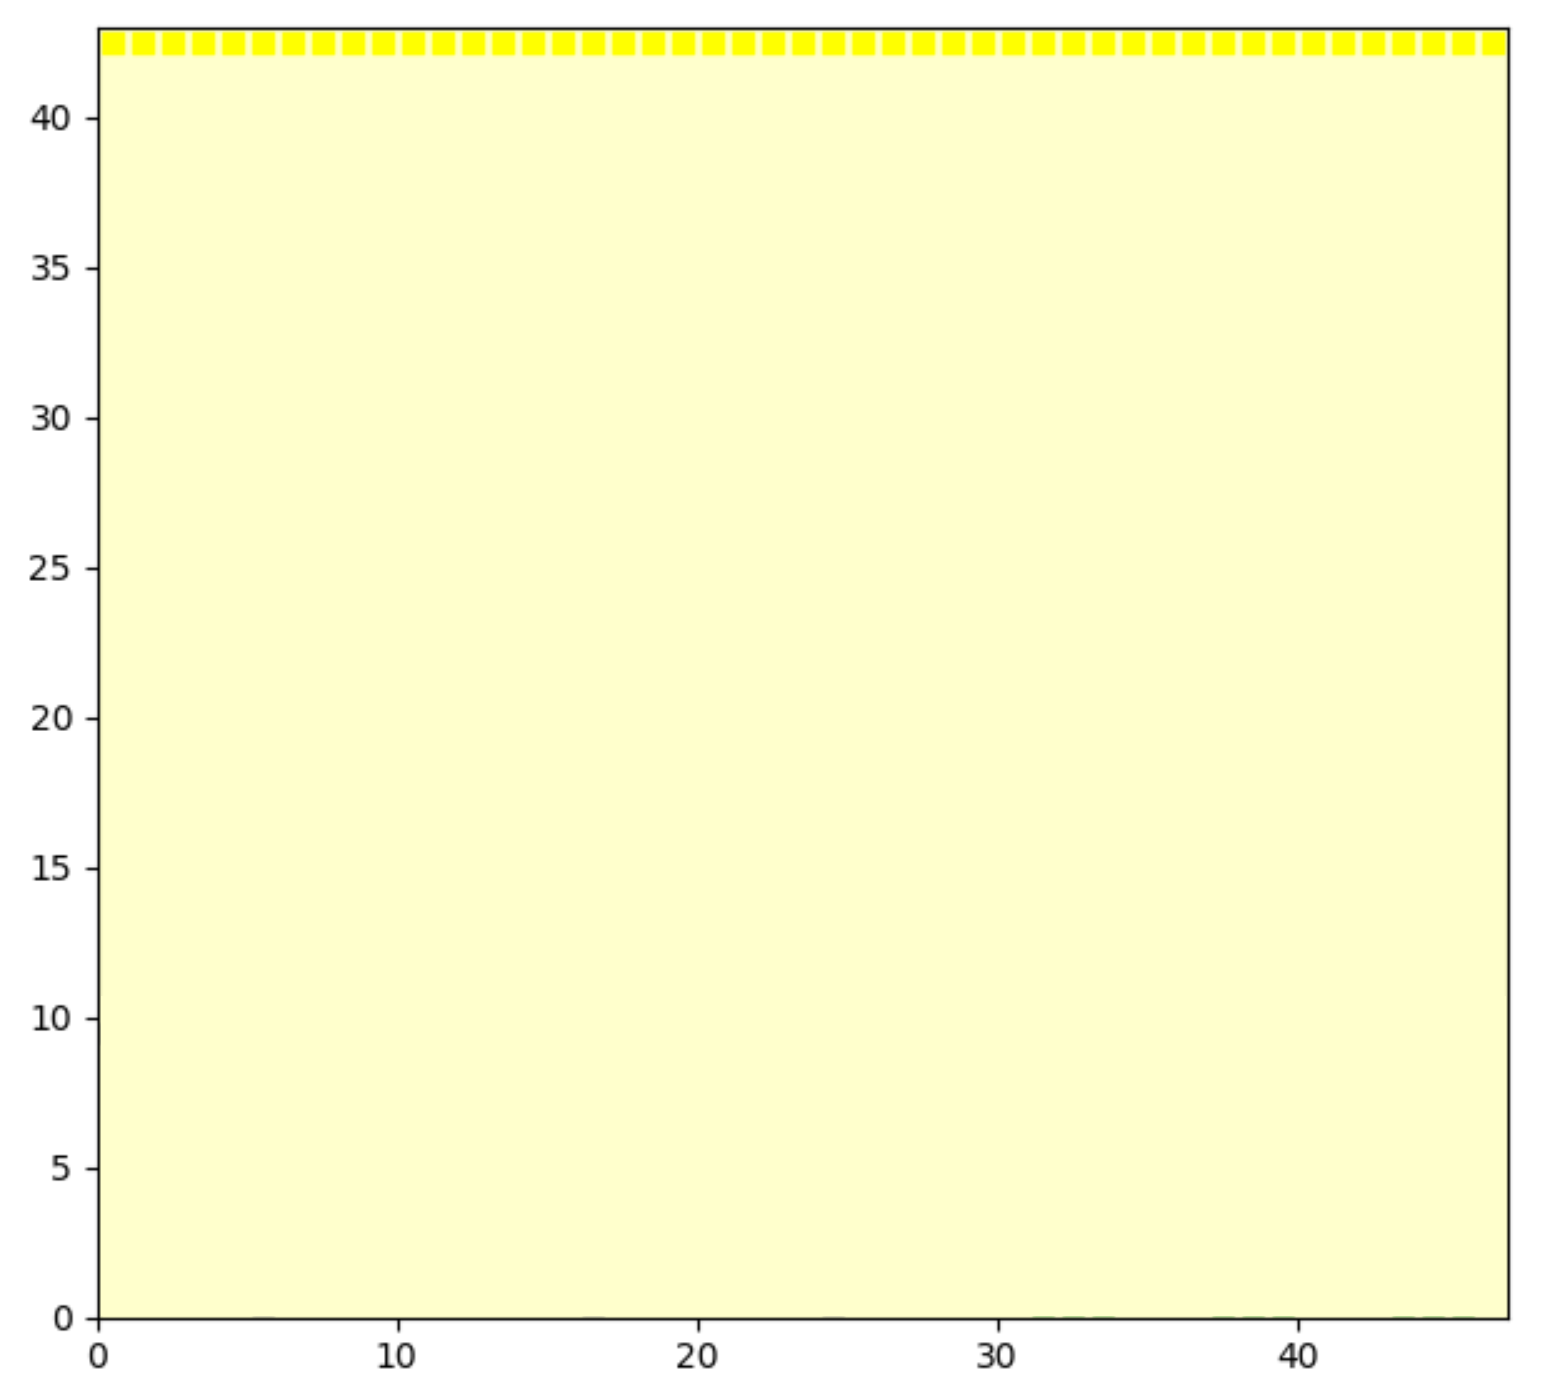
\includegraphics[width=\textwidth]{Figures/Map/ChargingStation.png}
\end{minipage}
\hspace{0.5cm}
\begin{minipage}[ht]{0.45\linewidth}
\centering
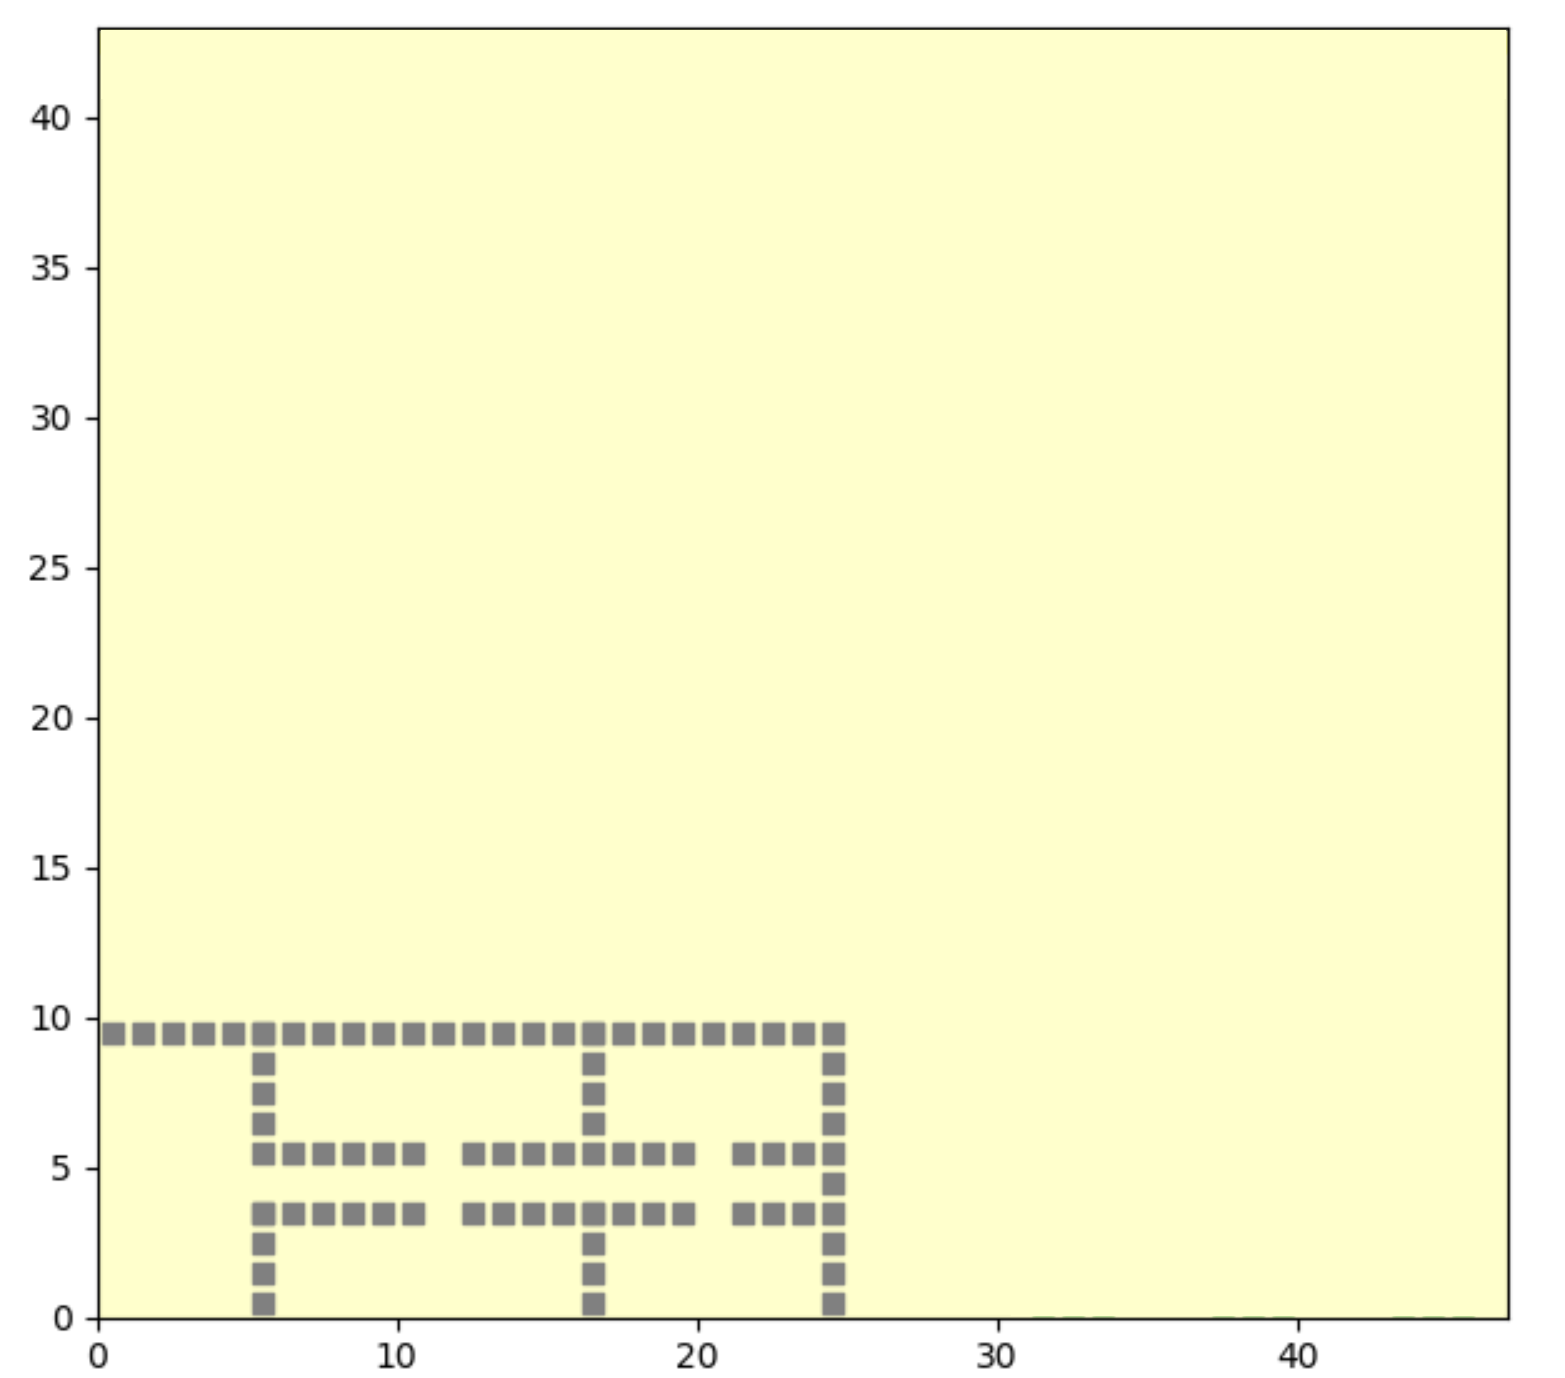
\includegraphics[width=\textwidth]{Figures/Map/Offices.png}
\end{minipage}

\begin{minipage}[ht]{0.45\linewidth}
\vspace{0.2cm}
\textbf{Area di ricarica:} Rappresentate con il colore giallo in alto all'interno dell'ambiente di simulazione. Durante questo lavoro sono state utilizzate solamente come punto di partenza degli AGV per la simulazione e per possibili lavori futuri.
\end{minipage}
\hspace{0.5cm}
\begin{minipage}[ht]{0.45\linewidth}
\vspace{0.2cm}
\textbf{Uffici:} Rappresentati con il colore grigio in basso a sinistra all'interno dell'ambiente di simulazione. Non hanno uno scopo effettivo bensì sono stati riportati per rimanere coerenti con la mappa originale del magazzino e non considerare spazi effettivamente non disponibili.
\end{minipage}

\newpage

\subsection{Modellazione agenti}
Ciascun agente definito all'interno della simulazione è caratterizzato da i seguenti attributi, che permettono la corretta gestione del sistema di simulazione e del comportamento degli agenti stessi:
\begin{itemize}
\item \textbf{Id:} un valore intero [1, 12] univoco associato a ciascun agente presente nella simulazione, permettendo il riconoscimento di ciascuno di essi.
\item \textbf{Colore:} un valore alfanumerico ["black"] che permette di rappresentare gli agenti con colori differenti all'interno della simulazione. Il simulatore attuale riporta tutti gli agenti con il colore nero.
\item \textbf{Posizione:} una coppia di numeri interi (x, y) che rappresenta la posizione dell'agente all'interno dell'ambiente di simulazione. Ciò permette di tener traccia della posizione di tutti gli agenti in qualsiasi momento della simulazione.
\item \textbf{Posizione iniziale:} una coppia di numeri interi (x, y) che rappresenta la posizione da cui l'agente è partito all'inizio della simulazione. Verosimilmente questa posizione dovrebbe coincidere con la posizione di una stazione di ricarica, e permetterebbe all'agente, una volta raggiunto il suo obiettivo, di tornare alla sua postazione di ricarica prestabilita. 
\item \textbf{Stato:} un valore alfanumerico che permette di capire cosa sta effettivamente facendo un certo agente. Questo attributo è fondamentale per la corretta elaborazione degli ordini e per lo svolgimento della simulazione. Nei seguenti paragrafi sono riportati gli stati assumibili da un agente [\ref{StatiAssumibili}] e le corrispettive transazioni possibili tra di essi [\ref{TransizioniStati}].
\item \textbf{Info sull'ordine:} un valore intero [-1, 200] che indica il numero dell'ordine su cui sta lavorando l'agente in quel determinato momento. Se il valore è pari a -1 vuol dire che l'agente non sta lavorando su nessun ordine in quel momento.
\item \textbf{Cliente:} un valore alfanumerico ["MI", "FI", "CO"] che indica la sigla del cliente dell'ordine che sta effettuando in un determinato momento. Ciò permette di determinare dove l'agente dovrà andare a scaricare l'ordine.
\item \textbf{Percorso:} una lista di coppie di valori interi [(x1, y1), (x2, y2), ... , (xN, yN)] che rappresenta il percorso calcolato e previsto dall'agente per raggiungere una determinata posizione (xN, yN) all'interno dell'ambiente di simulazione .
\item \textbf{Gate:} un valore alfanumerico [-1, 0, 1, 2] che rappresenta il gate a cui è diretto l'agente in quel momento. Ciascun gate è associato ad un determinato cliente, mentre il valore -1 significa che in quel momento l'agente non si sta dirigendo verso nessun gate. Ciò permette al sistema di gestione di controllare il flusso d'arrivo ai gate dei vari agenti.
\item \textbf{Goal:} un coppia di valori interi (x, y) che rappresenta la posizione all'interno dell'ambiente di simulazione che l'agente deve raggiungere in quel momento per compiere un'azione qualsiasi.
\item \textbf{Articoli prioritari:} una lista di valori alfanumerici ["Camicia", "Scarpa arancio", ... "Giubbetto"] che rappresenta il nome degli articoli che rappresenteranno una priorità assoluta per gli agenti in questione. Ciò permette di indirizzare un agente verso l'elaborazione di ordini contenti questi articoli rispetto ad altri ordini.

\end{itemize}

\subsubsection{Stati assumibili}\label{StatiAssumibili}
Come accennato nel paragrafo precedente, ciascun agente è caratterizzato da svariati attributi, tra cui uno che definisce lo stato in cui si trova l'agente in un determinato momento. Questo attributo ha un'estrema importanza per il corretto funzionamento della simulazione, in quanto regola il comportamento degli agenti in base allo stato in cui si trovano. \\
\noindent Di seguito è riportata la lista dei possibili stati che un agente può assumere durante il ciclo di vita di una simulazione insieme ad una breve descrizione per ciascuno di essi:
\begin{itemize}
    \item \textbf{Free}: un agente in questo stato non sta elaborando nessun ordine, rimanendo quindi disponibile ad essere impiegato per l'elaborazione di un ordine. Tutti gli agenti all'inizio di una simulazione si trovano in questo stato.
    \item \textbf{ToGoal}: un agente in questo stato ha in carico un determinato articolo da prelevare, quindi si starà muovendo verso il punto di prelievo associato all'articolo in questione. 
    \item \textbf{Loading}:  un agente in questo stato si trova fisicamente all'interno in uno dei punti di prelievi all'interno dell'ambiente di simulazione per caricare un determinato articolo. Una volta caricato l'articolo, prima di lasciare il punto di prelievo, calcola il percorso per arrivare al punto di scarico designato per l'articolo in questione.
    \item \textbf{ToGate}: un agente in questo stato ha in carico un articolo da scaricare presso un determinato gate, quindi si starà muovendo verso il punto di scarico del cliente designato.
    \item \textbf{ToWaitP}: un agente in questo stato ha in carico un articolo da scaricare presso un determinato gate ma, in quel determinato momento, il gate è occupato da altri agenti che stanno scaricando articoli, quindi si starà muovendo verso l'area di attesa.
    \item \textbf{Wait}:  un agente in questo stato ha in carico un articolo da scaricare presso un determinato gate e si trova già all'interno di un'area di attesa dato che il gate interessato è attualmente occupato da altri agenti. Rimarrà quindi in attesa che si liberi un gate per poter andare a scaricare l'articolo prelevato.   
    \item \textbf{Unloading}:  un agente in questo stato si trova fisicamente all'interno in uno dei gate all'interno dell'ambiente di simulazione per scaricare un determinato articolo. Una volta scaricato l'articolo, prima di lasciare il gate, verifica la presenza di altri articoli da elaborare e, se esistono, calcola il percorso per arrivare al prossimo punto di prelievo altrimenti imposta il percorso per tornare al suo punto di parte iniziale.
    \item \textbf{ToHome}: un agente in questo stato ha completato gli ordini di sua competenza e si dirige verso la sua postazione di ricarica all'interno dell'ambiente di simulazione. 
    \item \textbf{Home}: un agente in questo stato si trova fisicamente presso la sua postazione di ricarica all'interno dell'ambiente di simulazione. Tutti gli agenti alla fine di una simulazione si trovano in questo stato.
\end{itemize}

\newpage

\subsubsection{Transizioni tra stati} \label{TransizioniStati}
Nel paragrafo precedente [\ref{StatiAssumibili}] sono stati riportati e descritti tutti gli stati assumibili da un qualsiasi agente durante l'esecuzione di una simulazione. Il seguente schema rappresenta tutte le possibili transazioni tra gli stati di un agente, andando a dare una chiara idea del possibile ciclo di vita di un agente durante un'intera simulazione.
\begin{figure}[ht]
\centering
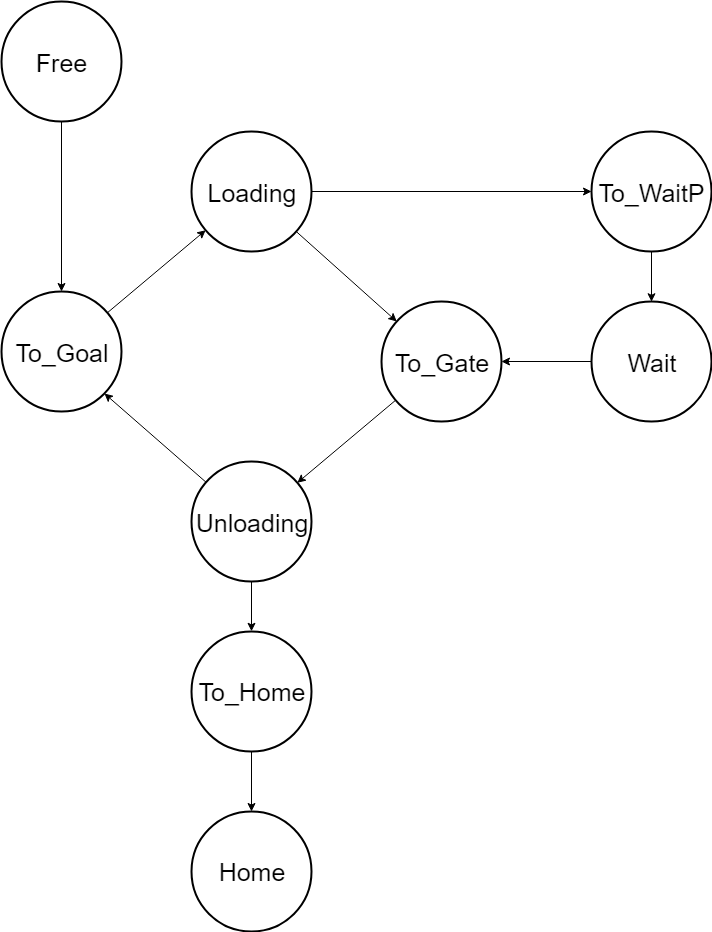
\includegraphics[width=0.75\textwidth,keepaspectratio]{Figures/Graphics/State_Transaction.png}
\caption[Transizioni tra stati di un agente]{Transazioni tra stati di un AGV}
\label{fig:TransizioniStati}
\end{figure}

\subsection{Gestione navigazione}
In questo lavoro si è deciso di sperimentare una navigazione libera da parte degli AGV, basandosi sulla loro capacità di visione attraverso sensori.\\
Si è scelto di prendere una decisione di questo genere per andare ad ottimizzare le distanze percorse dai singoli agenti, migliorando quindi durata della batteria, tempo di esecuzione dei task e usura delle componenti fisiche. Per fare ciò si è dovuto assumere che un sistema del genere non possa prevedere la presenza simultanea di impiegati umani e AGV all'interno del magazzino.\\

\noindent L'algoritmo utilizzato dagli AGV per la navigazione all'interno dell'ambiente di simulazione è l'algoritmo di Lee \cite{Lee}. Questo algoritmo, basato su BFS \cite{BFS}, viene solitamente utilizzato per calcolare il percorso da un punto ad un altro di un labirinto. 

\begin{figure}[ht]
\centering
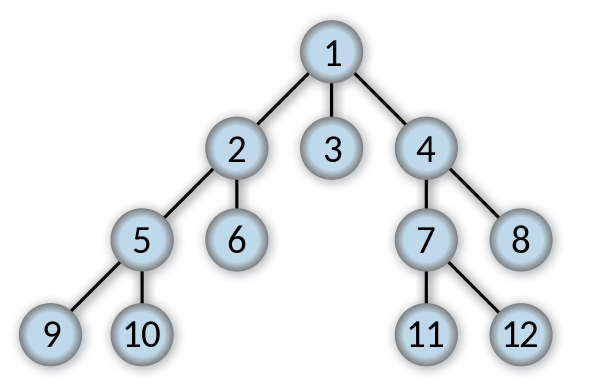
\includegraphics[width=0.75\textwidth,keepaspectratio]{Figures/Vario/BFS.png}
\caption[BFS: Ordine in cui i nodi vengono esplorati]{BFS: Ordine in cui i nodi vengono esplorati}
\label{fig:BFS}
\end{figure}

\noindent Permette infatti di ottenere sempre la soluzione migliore (se esiste), ma allo stesso tempo può essere lento e dispendioso in termini di memoria.
Si è deciso di utilizzare proprio questo algoritmo rispetto ad altri perchè l'ambiente di simulazione trattato in questo caso presenta delle dimensioni così ridotte che non è necessario andare ad ottimizzare la computazione in termini di tempo e memoria, andando ad ottener sempre la soluzione ottima senza richiedere una mole computazionale significativa.
\newpage

\subsubsection{Esempio navigazione - Libero}
\vspace{0.2cm}

\begin{minipage}[ht]{0.45\linewidth}
\centering
1) Posizioni iniziali
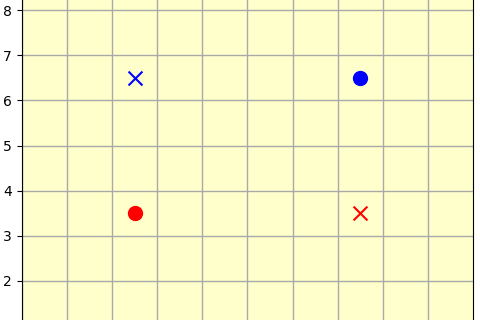
\includegraphics[width=\textwidth]{SimulazioniNavigazione/2AGV_NoConflitti/0.png}
\end{minipage}
\begin{minipage}[ht]{0.45\linewidth}
\centering
2) Sovrapposizione di intenzioni
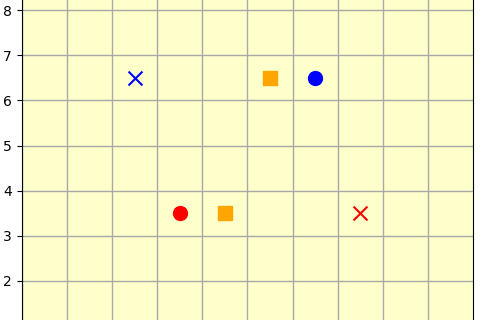
\includegraphics[width=\textwidth]{SimulazioniNavigazione/2AGV_NoConflitti/1.png}
\end{minipage}\\

\vspace{1cm}

\noindent \begin{minipage}[ht]{0.45\linewidth}
\centering
3) Ricalcolo percorso
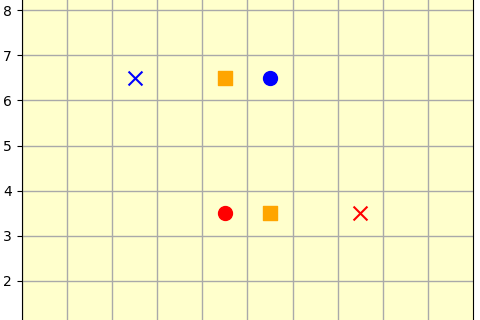
\includegraphics[width=\textwidth]{SimulazioniNavigazione/2AGV_NoConflitti/2.png}
\end{minipage}
\begin{minipage}[ht]{0.45\linewidth}
\centering
4) Navigazione
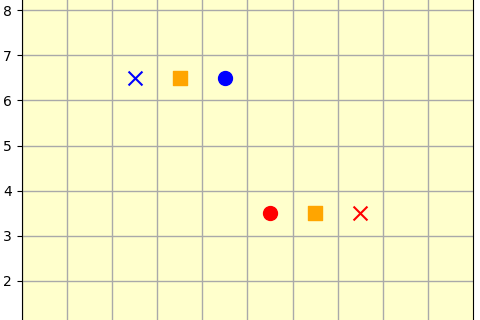
\includegraphics[width=\textwidth]{SimulazioniNavigazione/2AGV_NoConflitti/3.png}
\end{minipage}\\

\vspace{1cm}

\noindent \begin{minipage}[ht]{0.45\linewidth}
\centering
5) Navigazione
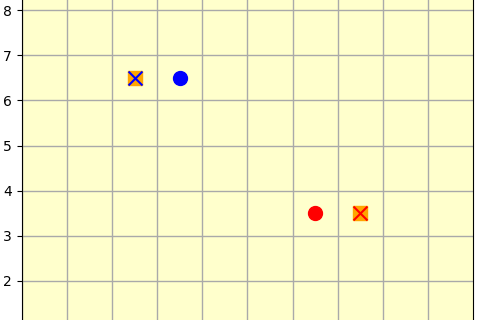
\includegraphics[width=\textwidth]{SimulazioniNavigazione/2AGV_NoConflitti/4.png}
\end{minipage}
\begin{minipage}[ht]{0.45\linewidth}
\centering
6) Obiettivo raggiunto
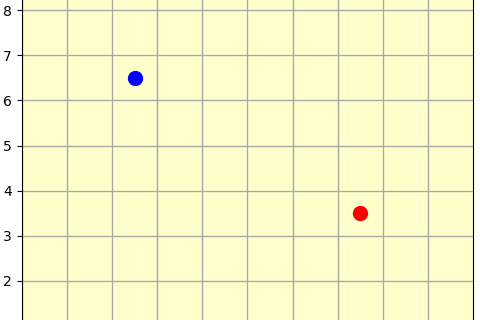
\includegraphics[width=\textwidth]{SimulazioniNavigazione/2AGV_NoConflitti/5.png}
\end{minipage}

\newpage

\subsubsection{Esempio navigazione - Ostacolo}
\vspace{0.2cm}

\begin{minipage}[ht]{0.45\linewidth}
\centering
1) Posizioni iniziali
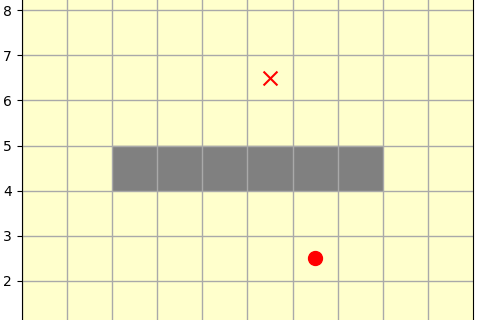
\includegraphics[width=\textwidth]{SimulazioniNavigazione/1AGV_Walls/0.png}
\end{minipage}
\begin{minipage}[ht]{0.45\linewidth}
\centering
2) Sovrapposizione di intenzioni
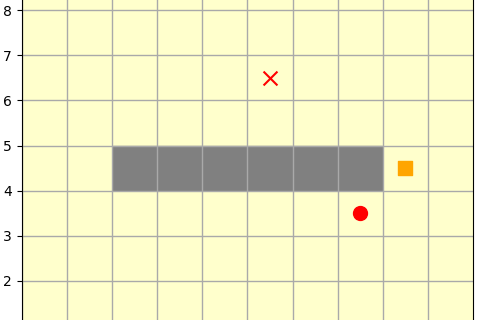
\includegraphics[width=\textwidth]{SimulazioniNavigazione/1AGV_Walls/1.png}
\end{minipage}\\

\vspace{1cm}

\noindent \begin{minipage}[ht]{0.45\linewidth}
\centering
3) Ricalcolo percorso
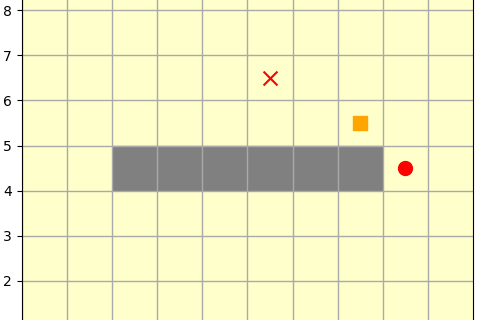
\includegraphics[width=\textwidth]{SimulazioniNavigazione/1AGV_Walls/2.png}
\end{minipage}
\begin{minipage}[ht]{0.45\linewidth}
\centering
4) Navigazione
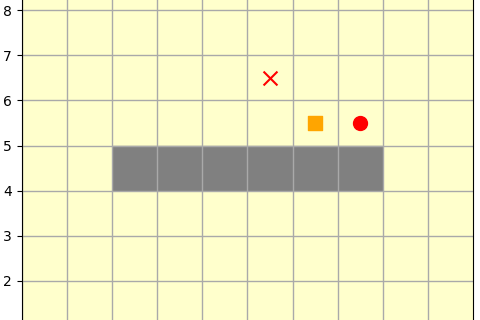
\includegraphics[width=\textwidth]{SimulazioniNavigazione/1AGV_Walls/3.png}
\end{minipage}\\

\vspace{1cm}

\noindent \begin{minipage}[ht]{0.45\linewidth}
\centering
5) Navigazione
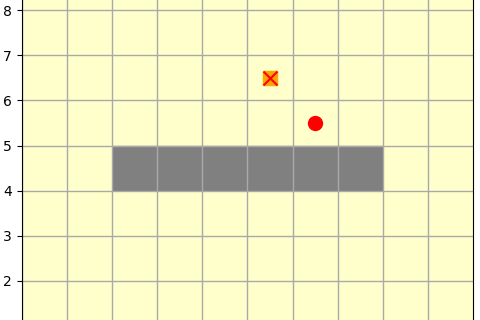
\includegraphics[width=\textwidth]{SimulazioniNavigazione/1AGV_Walls/4.png}
\end{minipage}
\begin{minipage}[ht]{0.45\linewidth}
\centering
6) Obiettivo raggiunto
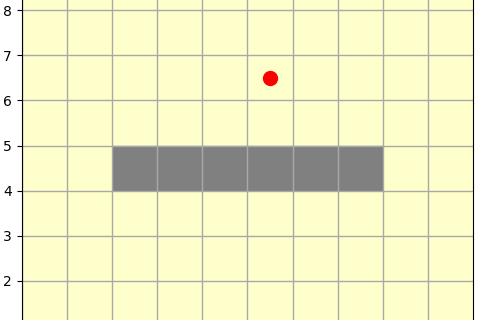
\includegraphics[width=\textwidth]{SimulazioniNavigazione/1AGV_Walls/5.png}
\end{minipage}

\newpage

\subsection{Gestione conflitti}
Il sistema di navigazione sopra descritto permette agli agenti di navigare in maniera ottimale su una mappa completamente statica, ciò che non varia nessun tipo di variazioni nel corso del loro percorso. Ovviamente un algoritmo di navigazione del genere porterebbe diverse problematiche, dato che durante la simulazione ci sono altri agenti che si muovono per l'ambiente. Proprio per questo motivo è stato necessario andare a progettare e realizzare un gestore dei conflitti di navigazione, in modo da risolvere qualsiasi problema potessero incontrare gli agenti durante il loro percorso.\\

\noindent Si definisce come "conflitto" la situazione in cui un agente si trova ad avere un ostacolo imminente sul suo percorso designato in precedenza, obbligandolo a dover ricalcolare il percorso. Le possibili soluzioni a questo problema sono principalmente due:\\
\begin{itemize}
\item L'agente sta fermo per uno step temporale, andando a controllare se lo step successivo persiste ancora lo stesso conflitto o meno.
\item L'agente ricalcola il percorso per arrivare alla sua destinazione, aggiungendo la posizione dove si è presentato il conflitto alla lista di posizioni non considerabili per la navigazione.
\end{itemize}

\newpage

\subsubsection{Esempio conflitto - Cambio direzione}
\vspace{0.2cm}

\begin{minipage}[ht]{0.45\linewidth}
\centering
1) Posizioni iniziali
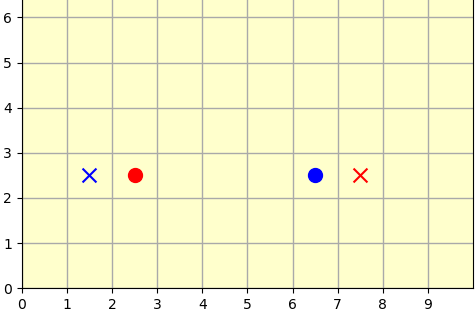
\includegraphics[width=\textwidth]{SimulazioniNavigazione/2AGV_ConflittoStandard/0.png}
\end{minipage}
\begin{minipage}[ht]{0.45\linewidth}
\centering
2) Sovrapposizione di intenzioni
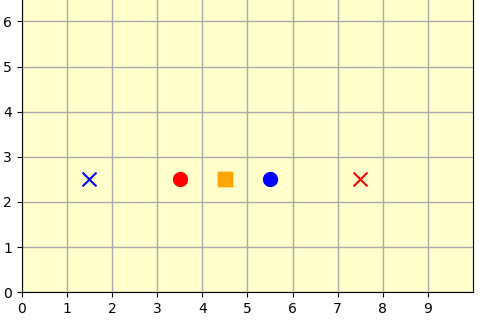
\includegraphics[width=\textwidth]{SimulazioniNavigazione/2AGV_ConflittoStandard/1.png}
\end{minipage}\\

\vspace{1cm}

\noindent\begin{minipage}[ht]{0.45\linewidth}
\centering
3) Ricalcolo percorso
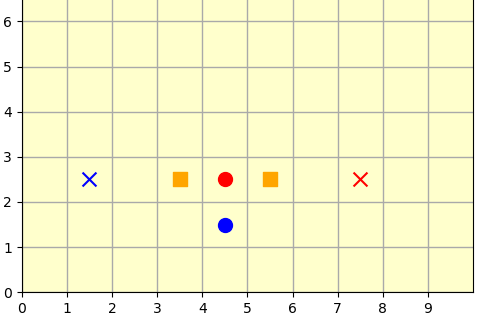
\includegraphics[width=\textwidth]{SimulazioniNavigazione/2AGV_ConflittoStandard/2.png}
\end{minipage}
\begin{minipage}[ht]{0.45\linewidth}
\centering
4) Navigazione
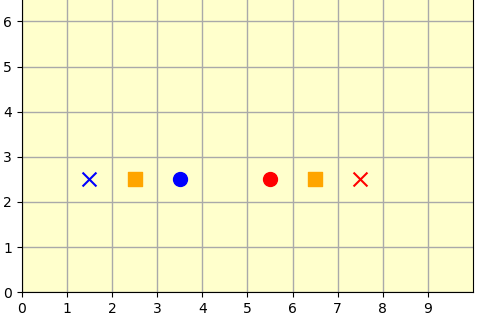
\includegraphics[width=\textwidth]{SimulazioniNavigazione/2AGV_ConflittoStandard/3.png}
\end{minipage}\\

\vspace{1cm}

\noindent\begin{minipage}[ht]{0.45\linewidth}
\centering
5) Navigazione
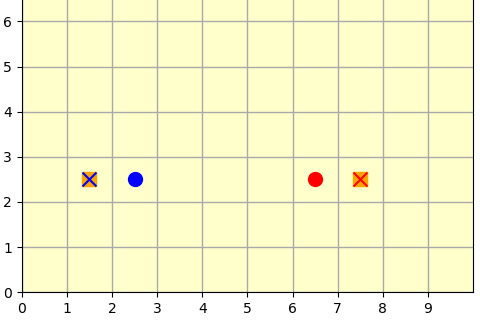
\includegraphics[width=\textwidth]{SimulazioniNavigazione/2AGV_ConflittoStandard/4.png}
\end{minipage}
\begin{minipage}[ht]{0.45\linewidth}
\centering
6) Obiettivo raggiunto
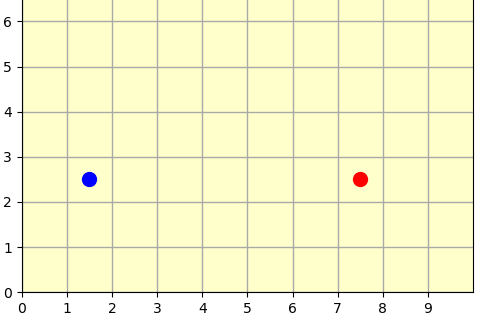
\includegraphics[width=\textwidth]{SimulazioniNavigazione/2AGV_ConflittoStandard/5.png}
\end{minipage}

\newpage

\subsubsection{Esempio conflitto - Attesa}
\vspace{0.2cm}

\begin{minipage}[ht]{0.45\linewidth}
\centering
1) Posizioni iniziali
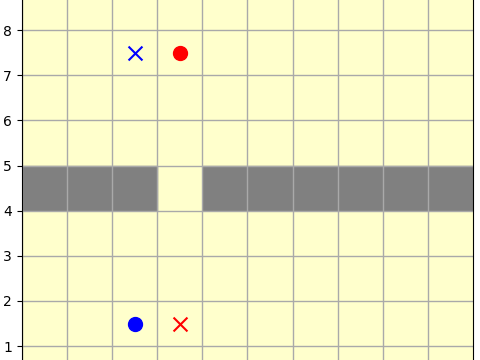
\includegraphics[width=\textwidth]{SimulazioniNavigazione/2AGV_ConflittoWait/0t.png}
\end{minipage}
\begin{minipage}[ht]{0.45\linewidth}
\centering
2) Sovrapposizione di intenzioni
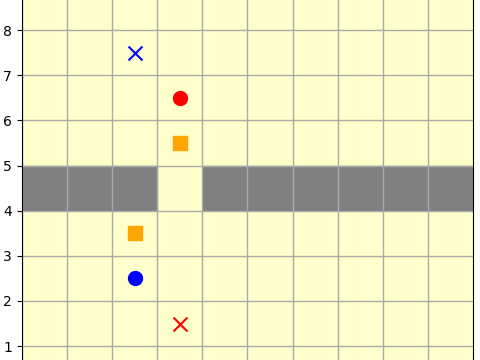
\includegraphics[width=\textwidth]{SimulazioniNavigazione/2AGV_ConflittoWait/1t.png}
\end{minipage}\\

\vspace{1cm}

\noindent \begin{minipage}[ht]{0.45\linewidth}
\centering
3) Ricalcolo percorso
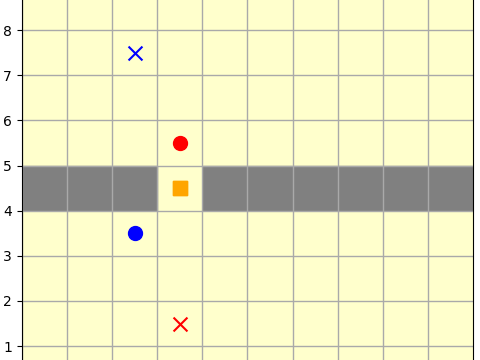
\includegraphics[width=\textwidth]{SimulazioniNavigazione/2AGV_ConflittoWait/2t.png}
\end{minipage}
\begin{minipage}[ht]{0.45\linewidth}
\centering
4) Navigazione
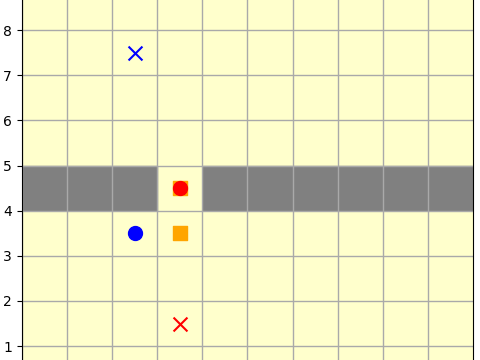
\includegraphics[width=\textwidth]{SimulazioniNavigazione/2AGV_ConflittoWait/3t.png}
\end{minipage}\\

\vspace{1cm}

\noindent\begin{minipage}[ht]{0.45\linewidth}
\centering
5) Navigazione
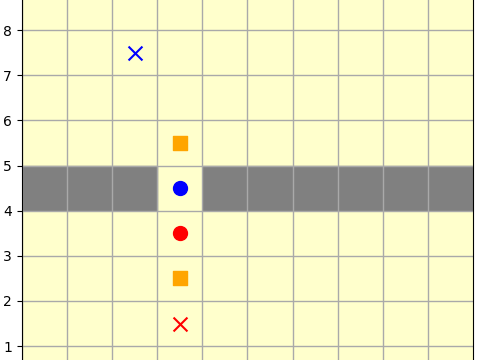
\includegraphics[width=\textwidth]{SimulazioniNavigazione/2AGV_ConflittoWait/4t.png}
\end{minipage}
\begin{minipage}[ht]{0.45\linewidth}
\centering
6) Navigazione..
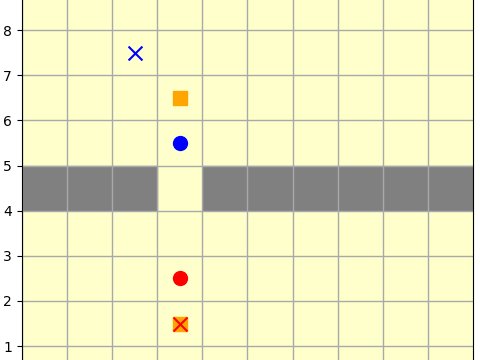
\includegraphics[width=\textwidth]{SimulazioniNavigazione/2AGV_ConflittoWait/5t.png}
\end{minipage}

\newpage

\subsection{Gestione area scarico merci}
Come rappresentato nel simulatore [\ref{ambienteSimulatore}] sono presenti tre punti di scarico detti "gates". Queste locazioni sono dove gli AGV devono scaricare gli articoli prelevati all'interno del magazzino. Considerando che gli ordini in input sono indirizzati verso tre destinazioni (MI, FI, CO), si è ipotizzato e deciso di assegnare a ciascun gate una specifica destinazione. 

\begin{figure}[H]
\centering
\includegraphics[width=0.5\textwidth]{Figures/Map/gates2.png}
\caption{Area scarico merci: MI, FI, CO}
\end{figure}

\noindent Inoltre, ciascun gate presenta solamente tre aree di scarico merci per gli AGV: una volta che una di queste aree di scarico merci viene occupata da un certo ordine, quest'ultimo deve essere portato a termine prima di poter essere nuovamente occupata con un nuovo ordine.

\subsection{Gestione area di atttesa}
Si è deciso di collocare due zone di attesa di fronte ai gates, ciascuna delle quali ha sei postazioni di attesa per AGV. Quindi un agente entrerà in attesa se non sono presenti zone di scarico disponibili per il cliente associato all'articolo che sta elaborando. \\
L'uscita dalla fase di attesa è determinata esclusivamente dalla disponibilità di un punto di scarico associato al cliente interessato. Se dovesse capitare che più AGV in attesa concorrono per la stessa postazione di scarico che si è appena liberata verrà applicato il meccanismo FIFO (First In First Out), che permetterà agli agenti in attesa da maggior tempo di riprendere l'elaborazione dei proprio articoli in maniera corretta.
\newpage

\subsection{Gestione ordini e agenti}
\subsubsection{Behaviour type 1}
Questo metodo fa si che ciascun AGV, una volta preso in carico un ordine, lo inizierà e lo porterà a termina in maniera autonoma. Non è previsto nessun tipo di collaborazione e/o concorrenza. La presa in carico degli ordine è puramente sequenziale. 

\subsubsection{Behaviour type 2}
Questo metodo fa si che ciascun AGV possa elaborare solamente un certo sottoinsieme degli articoli presenti all'interno del magazzino, come ad esempio una singola corsia oppure una categoria di articoli. Succederà quindi che un AGV andrà a lavorare su tutti quegli ordini che necessitano uno o più articoli di quelli da lui processabili. Ciò permette di ottenere un buon livello di collaborazione tra agenti, in quanto ciascuno si occupa di una parte dell'ordine, ma crea anche degli episodi di concorrenza per quanto riguarda la condivisione delle porte di scarico.

\subsubsection{Behaviour type 3}
Questo metodo fa si che ciascun AGV possa elaborare un qualsiasi articolo di un qualsiasi ordine in maniera puramente sequenziale. Un AGV andrà quindi a prendere il primo ordine in cima alla lista degli ordini da svolgere e andrà ad elaborare il primo degli articoli che necessitano ancora. Questo metodo di gestione crea una forte collaborazione tra agenti che, in base alle dimensioni di un ordine e non agli articoli al suo interno, possono collaborare tutti insieme su un singolo ordine.
\newpage
%%%%%%%%%%%%%%%%%%%%%%%%%%%%%%%%%%%%%%%%%%%%%%%
% AImplementazione
%%%%%%%%%%%%%%%%%%%%%%%%%%%%%%%%%%%%%%%%%%%%%%%
\section{Implementazione simulatore} 
\subsection{Interfaccia simulatore}
Il sistema di simulazione è stato interamente sviluppato tramite il linguaggio di programmazione Python, andando ad usufruire in particolare del modulo PycxSimulator.
Di seguito è riportata la struttura della schermata durante il ciclo di vita di una simulazione. I tasti sulla destra permettono all'utente di incominciare, finire o mettere in pausa la simulazione, mentre i grafici sulla sinistra permettono di monitorare la simulazione stessa e i relativi dati.
\begin{figure}[h]
\centering
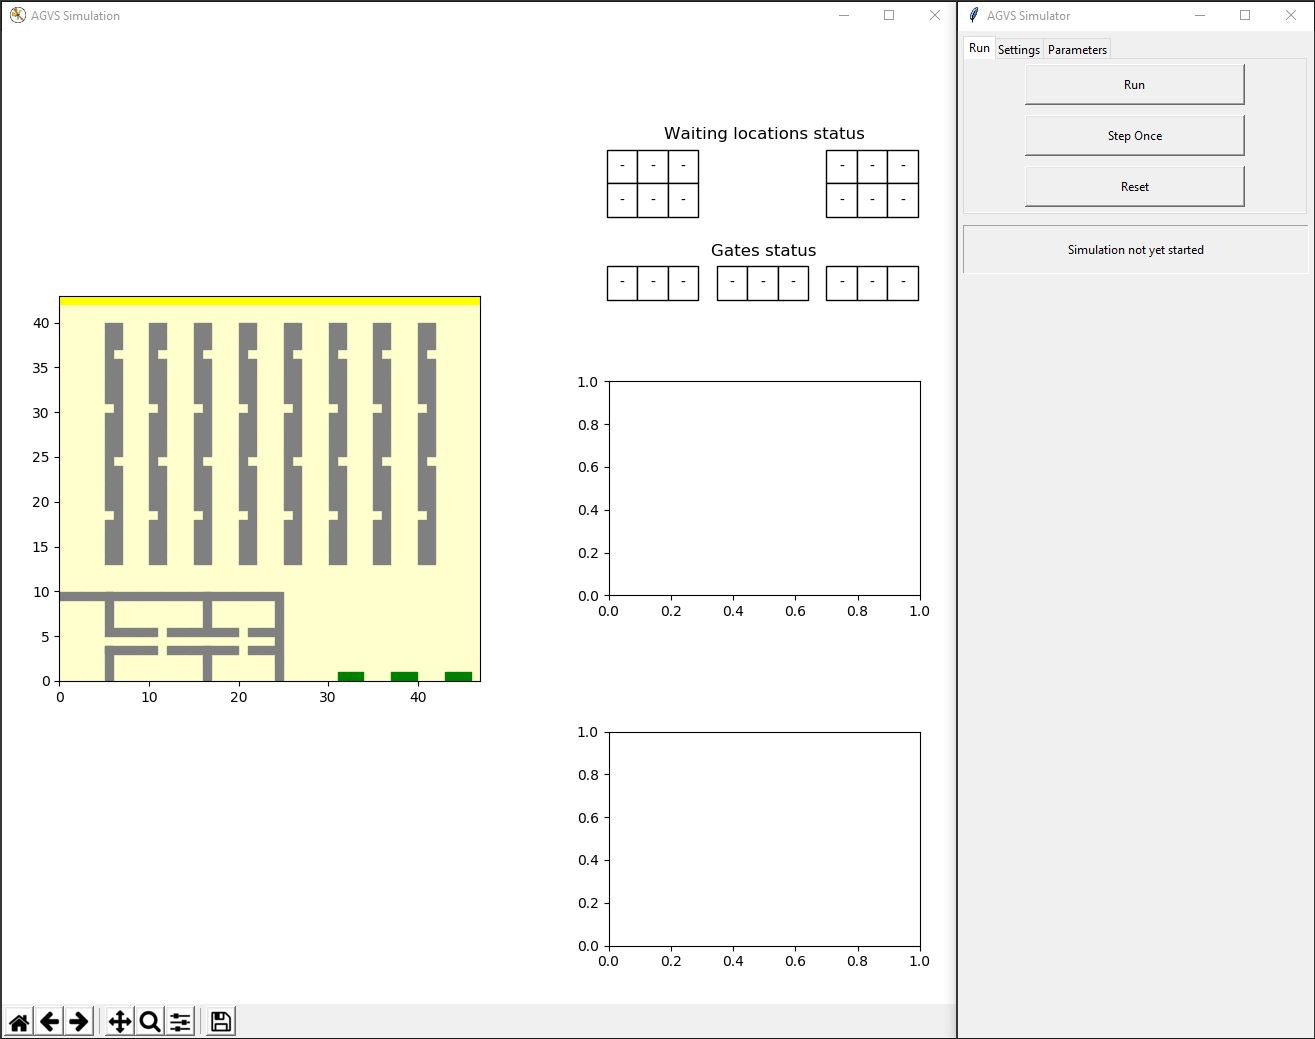
\includegraphics[width=1\textwidth,height=\textheight,keepaspectratio]{Figures/GUI/Simulatore.jpg}
\caption[GUI del simulatore implementato]{GUI del simulatore implementato}
\label{fig:Simulatore}
\end{figure}

\newpage

\begin{minipage}[ht]{0.45\linewidth}
\textbf{Settings:} dalla tab "settings" della schermata di gestione è possibile scegliere con quale intervallo di step temporali far aggiornare i grafici e l'ambiente relativi alla simulazione.
\vspace{0.3cm}
\end{minipage}
\hspace{0.5cm}
\begin{minipage}[ht]{0.45\linewidth}
\textbf{Parameters:} dalla tab "parameters"della schermata di gestione è possibile scegliere con quale parametri avviare la simulazione (Behaviour type e numero di AGV) tra quelli predefiniti:
\vspace{0.3cm}
\end{minipage}

\begin{minipage}[ht]{0.45\linewidth}
\centering
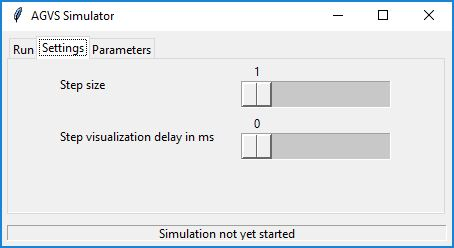
\includegraphics[width=\textwidth]{Figures/GUI/Console2.jpg}
\end{minipage}
\hspace{0.5cm}
\begin{minipage}[ht]{0.45\linewidth}
\centering
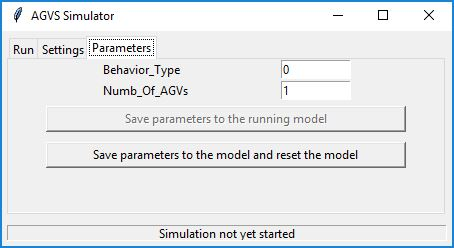
\includegraphics[width=\textwidth]{Figures/GUI/Console3.jpg}
\end{minipage}

\vspace{0.5 cm}

\noindent Durante l'esecuzione di una simulazione, come già detto in precedenza, i grafici riportati nella GUI del simulatore permettono all'utente di monitorare il ciclo di vita e lo sviluppo di una simulazione. L'immagine \ref{fig:SimulatoreEsec} riporta un esempio di tutto ciò che viene riportato graficamente durante il processo.
\begin{figure}[H]
\centering
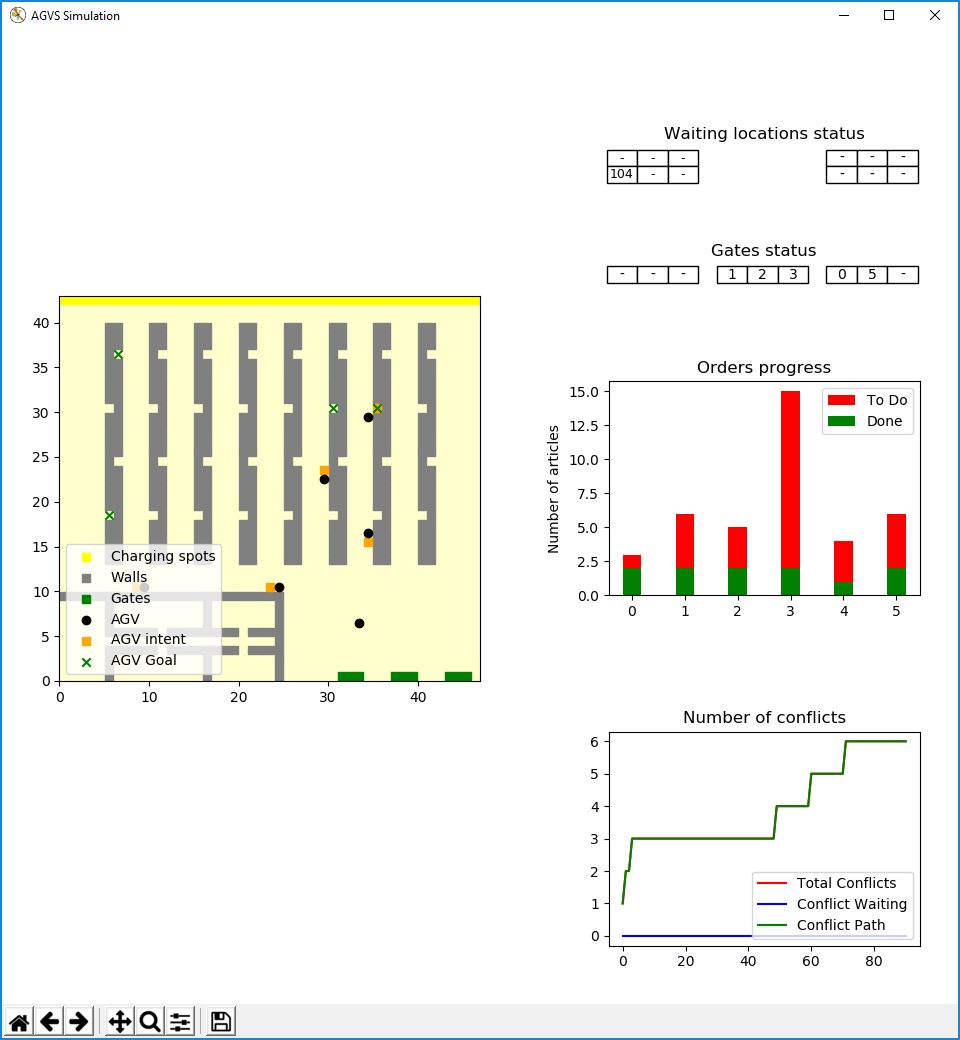
\includegraphics[width=0.6\textwidth,height=\textheight,keepaspectratio]{Figures/GUI/Simulatore_run2.jpg}
\caption[GUI del simulatore durante esecuzione]{GUI del simulatore  durante esecuzione}
\label{fig:SimulatoreEsec}
\end{figure}

\newpage
%%%%%%%%%%%%%%%%%%%%%%%%%%%%%%%%%%%%%%%%%%%%%%%
% Simulazione 
%%%%%%%%%%%%%%%%%%%%%%%%%%%%%%%%%%%%%%%%%%%%%%%
\section{Simulazione} % Main chapter title
Dopo aver progettato l'AGVS ed implementato il sistema di simulazione, si è passati alla fase di simulazione. Questa fase si pone l'obiettivo di simulare il funzionamento degli agenti con diverse configurazioni di comportamento, tenendo invariato il set di ordini in input. Ciò fornisce la possibilità di raccogliere dati e statistiche che permettono di effettuare un analisi complessiva delle performance del sistema con diverse configurazioni.

\subsection{Configurazioni simulate}
In particolare, si è deciso di eseguire la simulazione su 12 diverse configurazione in modo da poter andare ad analizzare i risultati al variare del comportamento e del numero di AGV. Le configurazioni eseguite sono state:
\begin{itemize}
\setlength\itemsep{0.1em}
    \item \textbf{BT1 A3:} Behaviour type 1 - Number of AGV 3 
    \item \textbf{BT1 A6:} Behaviour type 1 - Number of AGV 6 
    \item \textbf{BT1 A9:} Behaviour type 1 - Number of AGV 9
    \item \textbf{BT1 A12:} Behaviour type 1 - Number of AGV 12
    \vspace{0.3cm}
    \item \textbf{BT2 A3:} Behaviour type 2 - Number of AGV 3
    \item \textbf{BT2 A6:} Behaviour type 2 - Number of AGV 6 
    \item \textbf{BT2 A9:} Behaviour type 2 - Number of AGV 9 
    \item \textbf{BT2 A12:} Behaviour type 2 - Number of AGV 12 
    \vspace{0.3cm}
    \item \textbf{BT3 A3:} Behaviour type 3 - Number of AGV 3 
    \item \textbf{BT3 A6:} Behaviour type 3 - Number of AGV 6
    \item \textbf{BT3 A9:} Behaviour type 3 - Number of AGV 9 
    \item \textbf{BT3 A12:} Behaviour type 3 - Number of AGV 12 
    
\end{itemize}

\newpage

\subsection{Lista degli ordini per simulazione}
La lista di ordini considerata per effettuare le diverse simulazioni del sistema è stata scelta in maniera semi arbitraria. Come prima cosa è stato indispensabile aggregare articoli appartenente a classi diverse nella stessa classe oppure al contrario dividere una singola classe di articoli in più sottoclassi. Tutto ciò ha permesso di ottenere un numero di classi adeguato alla simulazione sul sistema implementato. \newline
Successivamente si sono selezionati N ordini casuali da quelli disponibili, mantenendo invariate le distribuzioni di classi degli articoli all'interno di essi.\\

\noindent E' possibile notare come gli ordini che indirizzati al cliente "CO" sono di gran lunga più numerosi rispetto a quelli indirizzati a "FI" e "MI": questo rispecchia la distribuzione di ordini suddivisi per cliente presente all'interno degli ordini realmente raccolti dalla logistica.

\begin{figure}[H]
\centering
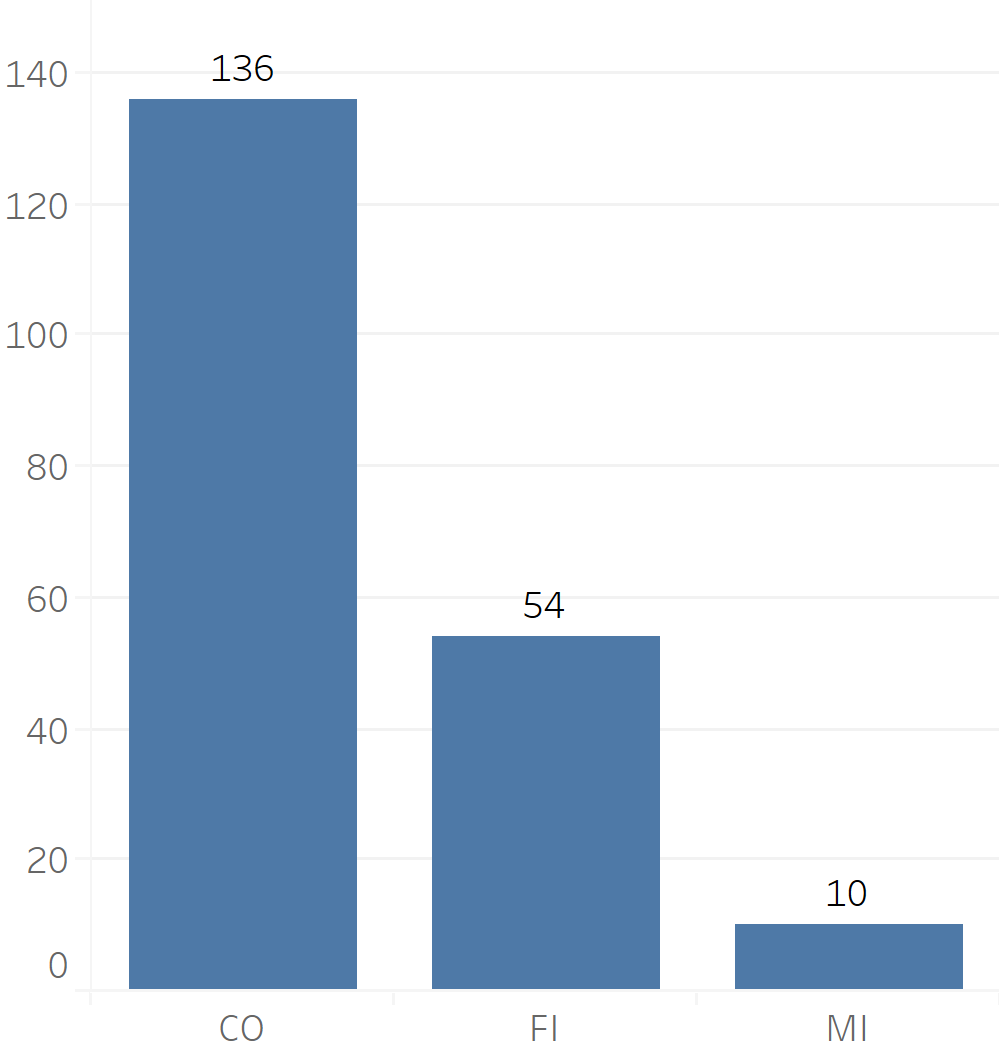
\includegraphics[width=0.7\textwidth,keepaspectratio]{Figures/Graphics/Orders_simulation.png}
\captionof{figure}[Numero di ordini associati ad ogni cliente]{Numero di ordini associati ad ogni cliente.}
\label{fig:OrdiniSimulazione}
\end{figure}

\noindent Inoltre è possibile vedere dal seguente grafico come alcuni articoli compaiono molto più spesso all'interno di determinati clienti rispetto ad altri. 
\noindent Tutto ciò è stato mantenuto di proposito all'interno della lista degli ordini utilizzata per le simulazioni in modo tale da renderla il più verosimile possibile e andare a considerare tutte quelle esigenze realmente presenti all'interno del contesto analizzato.

\begin{figure}[H]
\centering
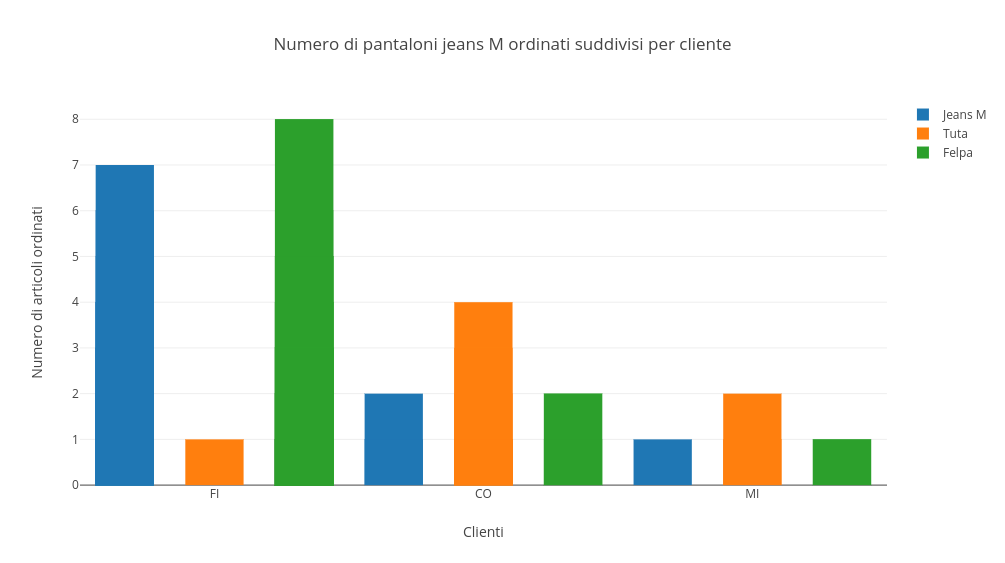
\includegraphics[width=1\textwidth,keepaspectratio]{Figures/Graphics/articoli_clienti.png}
\caption[Numero di diversi articoli per cliente]{Numero di diversi articoli ordinati per cliente}
\label{fig:Electron}
\end{figure}



\newpage

\subsection{Metriche di valutazione} \label{MetricheValutazione}
Per poter valutare le performance delle configurazione simulate è stato realizzato un sistema di raccolta dati che ha permesso di raccogliere diverse informazioni, tra cui:

\begin{itemize}
    \item \textbf{Conflicts:} numero di conflitti che sono stati rilevati durante la configurazione per ogni singolo AGV.
    \item \textbf{Conflict Wait:} numero di conflitti che sono stati rilevati durante la configurazione per ogni singolo AGV e che sono stati risolti con un AGV in attesa per un turno.
    \item \textbf{Conflict Path:} numero di conflitti che sono stati rilevati durante la configurazione per ogni singolo AGV e che sono stati risolti con un AGV che ricalcola il percorso per la sua destinazione.
    \item \textbf{Waiting Gate:} numero di timestep trascorsi da ciascun AGV all'interno delle aree di attesa.
    \item \textbf{Articles:}  numero di articoli elaborati, e quindi portati ad uno specifico gate, da ciascun AGV.
    \item \textbf{Moving Steps:} numero di step, ovvero di spostamenti da una cella ad un'altra adiacente, di ciascun AGV.
\end{itemize}

\noindent Questi parametri sono stati raccolti ad ogni timestep della simulazione per ogni singolo AGV per ogni configurazione, così da poter analizzare i risultati che si otterrano secondo diversi punti di vista.


\newpage
%%%%%%%%%%%%%%%%%%%%%%%%%%%%%%%%%%%%%%%%%%%%%%%
% Analisi dei risultati 
%%%%%%%%%%%%%%%%%%%%%%%%%%%%%%%%%%%%%%%%%%%%%%%
\section{Analisi dei risultati}
Una volta raccolti i dati inerenti alle diverse simulazioni, si è passati ad analizzarli, con lo scopo di determinare la configurazione migliore: prima di procedere è indispensabile però dare una definizione di "configurazione migliore". \\

\noindent Sicuramente una configurazione può essere considerata più performante di un'altra se impiega meno tempo per portare a termine la stessa mole di lavoro. Andando però a consideraro solo il tempo impegato si trascurano alcuni aspetti che sono indispensabili per un'attività reale come in questo caso. E' infatti indispensabile trovare anche un giusto compromesso sul numero di AGV, dato che rappresentano un costo non indifferente di acquisto e mantenimento da parte delle aziende. \\

\noindent Lo scopo di questa fase quindi è proprio quello di individuare come i parametri delle configurazioni influiscono sulle performance del sistema, in modo tale da poter trovare la configurazione migliore tenendo ben presente il contesto lavorativo ed economico in cui questo lavoro si colloca. \\
\noindent In questa sezione sono riportati, descritti e analizzati alcuni grafici rappresentativi dei dati raccolti durante la fase di simulazione e che sono stati considerati più rilevanti. In particolare si andrà ad analizzare:\\

\begin{itemize}
\item Timestep per ciascuna configurazione
\item Conflitti per ciascuna configurazione
\item Articoli elaborati da ciascun AGV
\item Timestep di attesa per ciascun AGV
\end{itemize}

\newpage
\subsection{Analisi generale delle configurazioni}
\subsubsection{Timestep per ciascuna configurazione}
Come prima cosa si è andati ad analizzare il tempo richiesto da ciascuna configurazione per elaborare la lista di ordini simulata, essendo questa una metrica di valutazione fondamentale per una possibile implementazione reale del sistema. Il seguente grafico riporta il tempo totale richiesto da ciascuna delle 12 diverse simulazioni avviate. \\

\noindent Andando ad analizzare le configurazioni testate con 3 AGV si può vedere come i tempi richiesti dalle tre diverse simulazioni non presentano grandi differenze tra loro. E' possibile notare, pero, come all'aumentare del numero di AGV questa differenza aumenta significativamente, con le configurazioni testate con BT3 che presentano tempi totali largamente inferiori rispetto alle altre configurazioni testate.

\begin{figure}[H]
\centering
  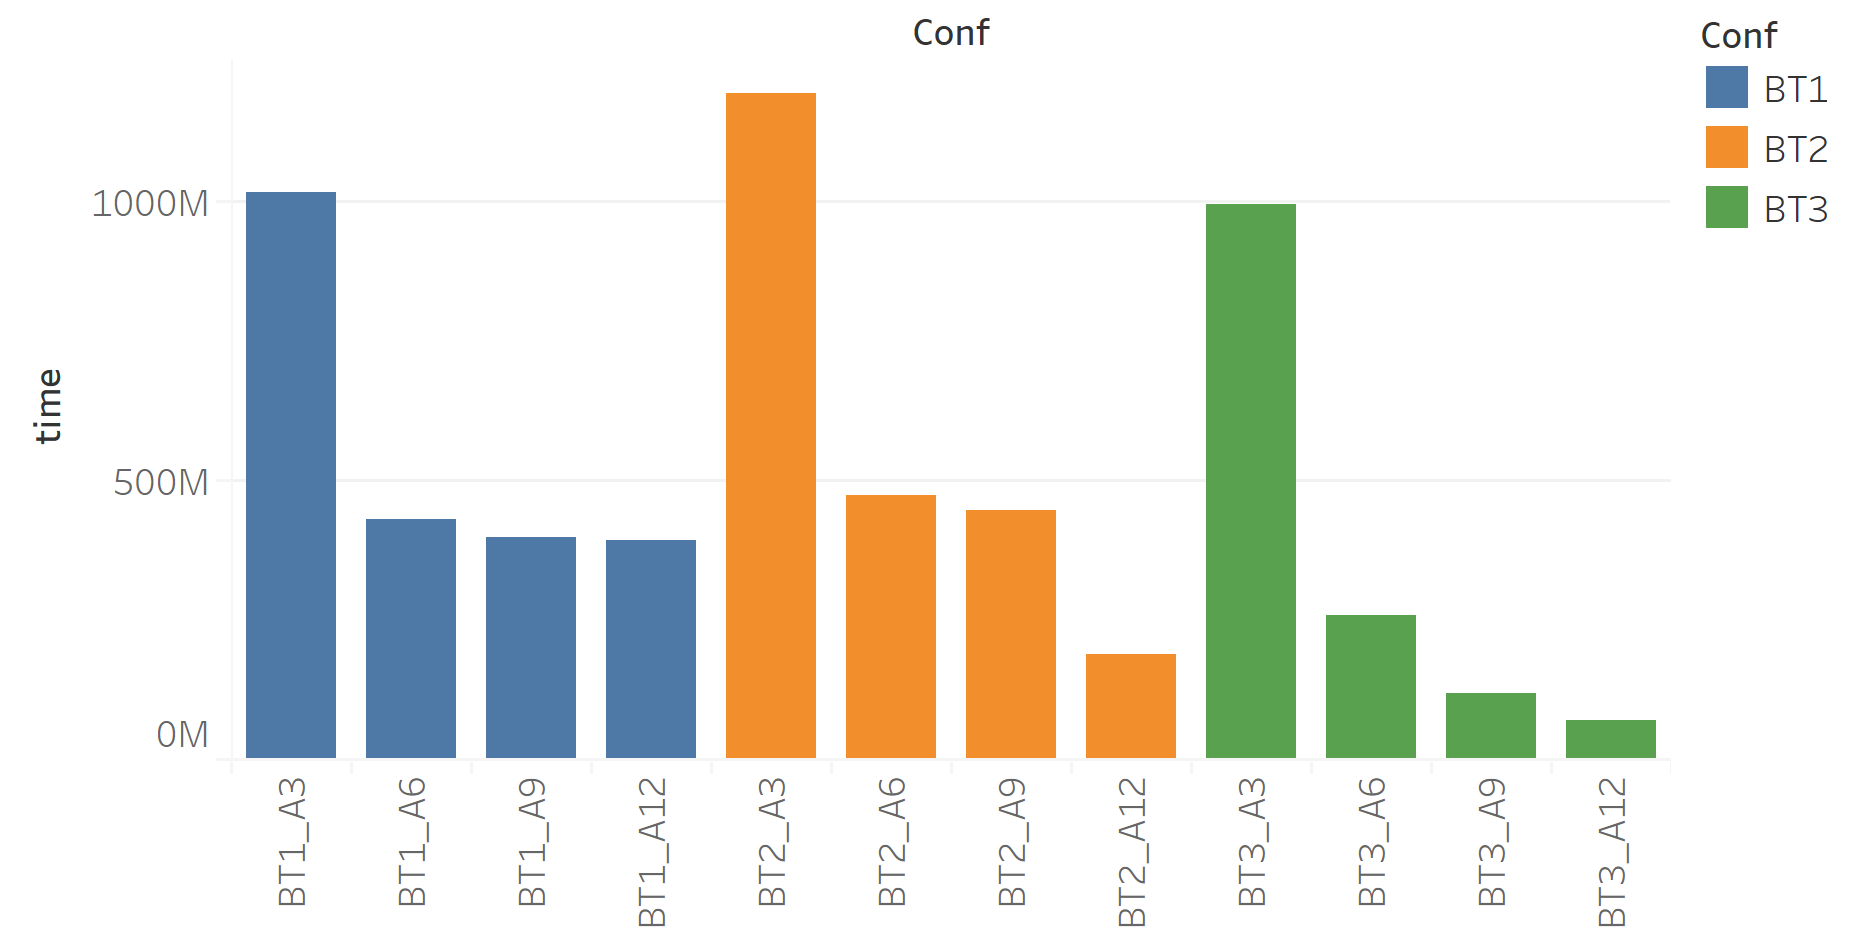
\includegraphics[width=1\linewidth]{Figures/Results_Graphics/Time_Total.png}
  \caption{Tempo necessario al completamento degli ordini per ciascuna configurazione}\label{fig:articles_agv_bt1}
\end{figure}

\newpage

\subsubsection{Conflitti per ciascuna configurazione}
Un'altra metrica che deve essere presa sicuramente in considerazione per eventuali decisioni future di realizzazione del sistema è il numero totale di conflitti tra AGV successi durante il ciclo di vita di una simulazione.\\
Il seguente grafico riporta sull'asse delle ascisse il tempo richiesto dalla simulazione per terminare gli ordini e sull'asse delle ordinate il numero totale di conflitti. Si può andare ad identificare un forte rapporto inversamente proporzionale tra tempo richiesto al completo degli ordini in una certa configurazione e il relativo numero di conflitti avvenuti. Infatti, al diminuire del tempo richiesto si presenta un forte aumento del numero di conflitti. Questo rapporto è estremamente significativo su configurazioni con un alto numero di AGV, infatti il seguente grafico riporta le tre configurazioni testate con 12 agenti.
\begin{figure}[H]
\centering
  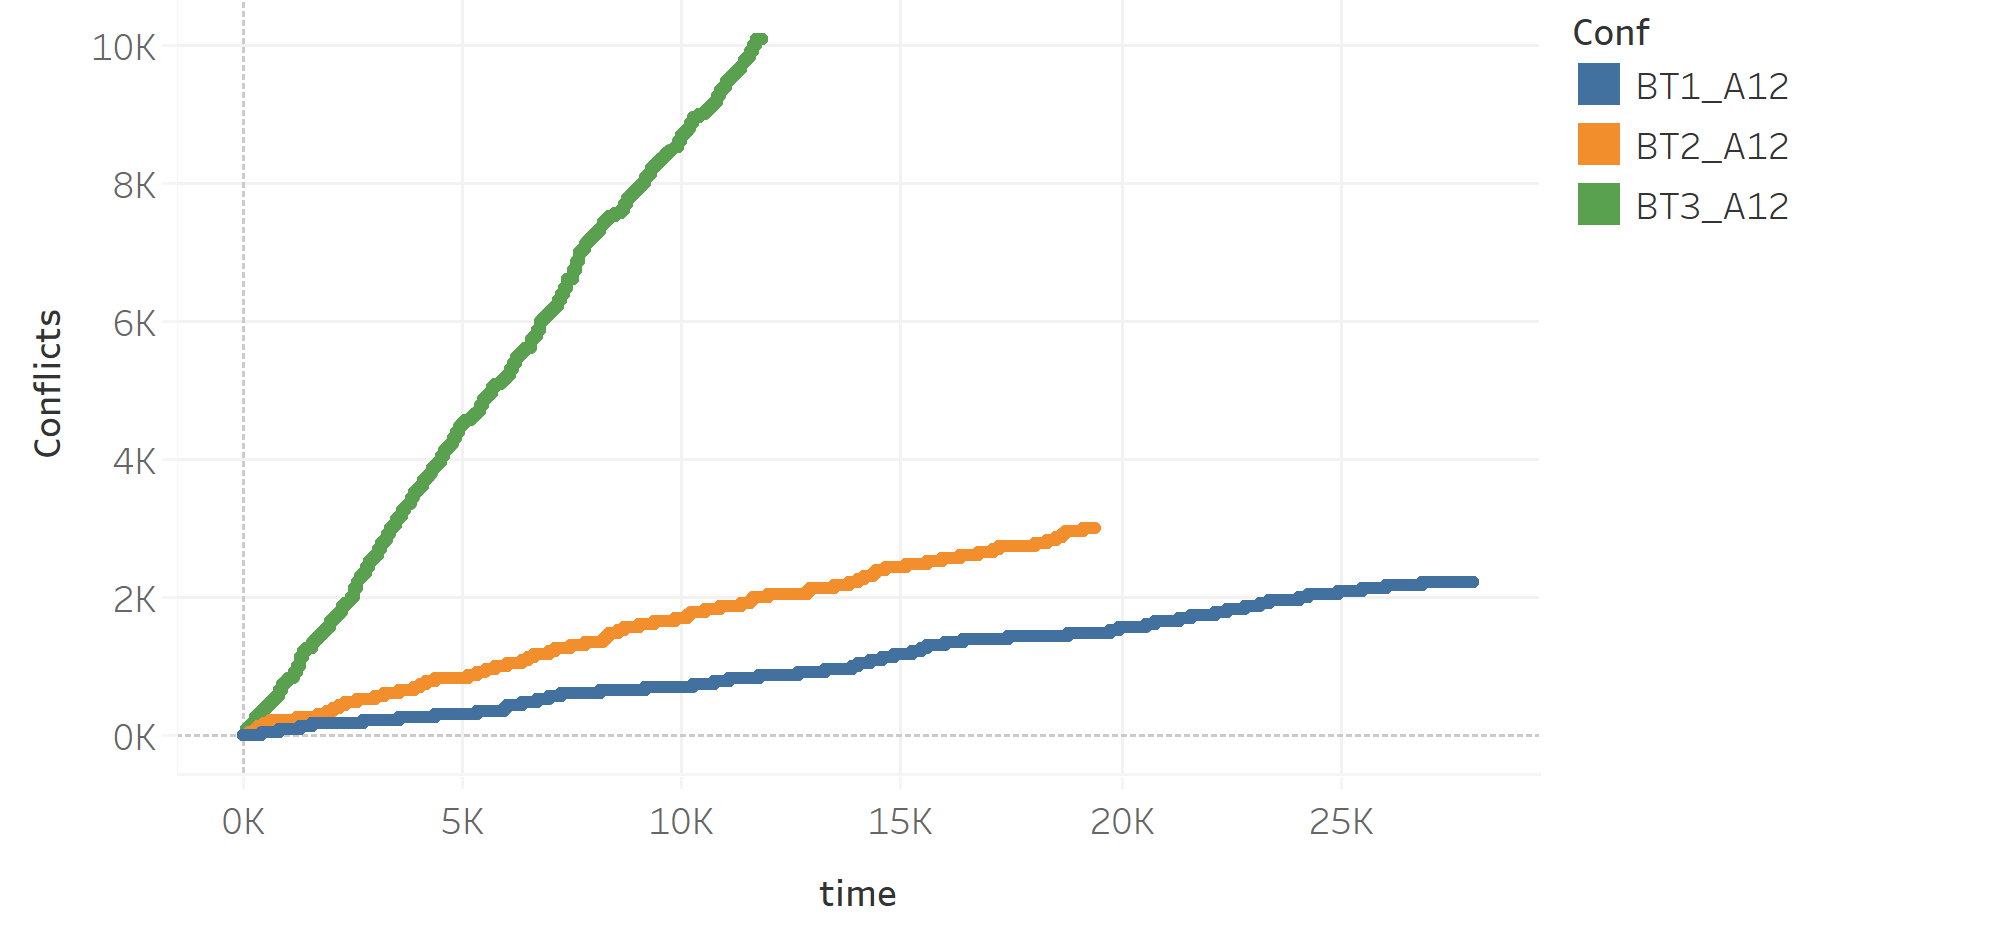
\includegraphics[width=1\linewidth]{Figures/Results_Graphics/Rapporto_tempoconflitti.png}
  \caption{Rapporto tra tempo richiesto e conflitti avvenuti in ciascuna configurazione}\label{fig:articles_agv_bt1}
\end{figure}

\newpage

\subsection{Analisi intra BT: timestep/conflitti}
Nel seguente paragrafo verranno mostrati e descritti i grafici inerenti al numero di timesteps e il relativo numero di conflitti avvenuti per ciascun Behaviour Type. In particolare, verrà analizzato il rapporto tra queste due metriche di valutazione all'aumentare del numero di AGV per ogni BT.

\subsubsection{Analisi BT 1}
Per quanto riguarda il BT1 si può notare la presenza di una forte diminuzione dei timestep solo tra le configurazioni che utilizzano rispettivamente 3 e 6 agenti. Infatti, pur aumentando il numero di agenti da 6 a 12, il numero totale di timestep richiesti rimane pressochè invariato a descapito però di un significativo aumento dei conflitti\\

\begin{figure}[H]
\centering
  \includegraphics[width=1\linewidth]{Figures/Results_Graphics/BT1_TimeConflicts.png}
  \caption{BT1: Confronto tra numero di conflitti e timestep richiesti}\label{fig:BT1_TimeConflicts}
\end{figure}

\subsubsection{Analisi BT 2}
Per quanto riguarda il BT2 invece si può notare come, all'aumentare del numero di AGV, si ottiene da una parte una diminuzione dei timestep richiesti e dell'altra parte un aumento del numero di conflitti, che risultano entrambi gli andamenti pressochè costanti.

\begin{figure}[H]
\centering
  \includegraphics[width=1\linewidth]{Figures/Results_Graphics/BT2_TimeConflicts.png}
  \caption{BT2: Confronto tra numero di conflitti e timestep richiesti}\label{fig:BT2_TimeConflicts}
\end{figure}

\subsubsection{Analisi BT 3}
Per quanto riguarda il BT3 invece si può notare come, all'aumentare del numero di AGV, le due metriche di valutazione rispecchiano pressochè un andamento inversamente proporzionale. Infatti, ad una significativa diminuzione del numero di timestep corrisponde un considerevole aumento del numero di conflitti.
\begin{figure}[H]
\centering
  \includegraphics[width=1\linewidth]{Figures/Results_Graphics/BT3_TimeConflicts.png}
  \caption{BT3: Confronto tra numero di conflitti e timestep richiesti}\label{fig:BT3_TimeConflicts}
\end{figure}

\newpage
\subsection{Altri fattori di analisi}
\subsubsection{Articoli elaborati da ciascun AGV}
\noindent I grafici sotto illustrati riportano il numero di articoli correttamente elaborati da ogni singolo AGV per ciascuna configurazione durante l'esecuzione della simulazione. Questa metrica è di estrema importanza in quanto permette di verificare se esistono differenze significative tra la mole di lavoro assegnata ad un AGV rispetto ad un altro all'interno della stessa simulazione.

\begin{figure}[H]
\centering
  \includegraphics[width=0.8\linewidth]{Figures/Results_Graphics/Articles_BT1.png}
  \caption{Numero di articoli elaborati da ciascun AGV con BT1}\label{fig:articles_agv_bt1}
\end{figure}

\noindent La BT1 [Fig \ref{fig:articles_agv_bt1}] mantiene un carico di lavoro bilanciato quando la simulazione è eseguita con un numero ridotto di AGV, per poi andare a perdere questa distribuzione equa nelle configurazioni con numerosi AGV.\\
\noindent Invece, come si può vedere di seguito, la configurazione BT2 [Fig \ref{fig:articles_agv_bt2}] presenta delle differenze significative per qualsiasi numero di AGV, mostrando degli agenti che, durante un singolo ciclo di simulazione, elaborano anche il doppio degli articoli elaborati da altri agenti nella stessa simulazione.

\begin{figure}[H]
\centering
  \includegraphics[width=0.8\linewidth]{Figures/Results_Graphics/Articles_BT2.png}
  \caption{Numero di articoli elaborati da ciascun AGV con BT2}\label{fig:articles_agv_bt2}
\end{figure}

\noindent Per quanto riguarda invece la BT3 [Fig \ref{fig:articles_agv_bt3}] si è rilevata di gran lunga la configurazione che meglio distribuisce la mole di lavoro tra gli AGV, indipendentemente dal numero di AGV operativi. Ciò permette non solo di ridurre il tempo di elaborazione totale degli ordini, ma anche di non sovraccaricare di lavoro un determinato agente che potrebbe danneggiarsi o richiedere manutenzione preventiva, che implicherebbero soldi e tempo.
 
\begin{figure}[H]
\centering
  \includegraphics[width=0.8\linewidth]{Figures/Results_Graphics/Articles_BT3.png}
  \caption{Numero di articoli elaborati da ciascun AGV con BT3}\label{fig:articles_agv_bt3}
\end{figure}

\newpage

\subsubsection{Timestep di attesa per ciascun AGV}
Un'altra metrica che ci ha permesso di raggiungere l'obiettivo di questo lavoro è il numero di step temporali passati in attesa da ciascun AGV di ogni simulazione avviata. Considerando il dominio su cui questo lavoro è stato svolto, una delle priorità maggiori è proprio quella di ottimizzare l'utilizzo delle risorse, andando quindi a minimizzare quei momenti in cui le risorse non sono operative. \\

\noindent Il seguente grafico riporta il numero di step temporali attesi da ciascun AGV nelle tre diverse BT durante la simulazione con 12 AGV.
\begin{figure}[H]
\centering
  \includegraphics[width=1\linewidth]{Figures/Results_Graphics/Waiting.png}
  \caption{Numero di step temporali passati in attesa da ciascun AGV per i tre diversi BT}\label{fig:waiting_bt_a12}
\end{figure}

\noindent Come risulta visibile dal grafico sopra riportato la differenza tra il numero di step attesi da ciascun AGV durante le prime due configurazioni comparate con la BT3 è enorme. La BT3 infatti tende ad azzerare il numero di step spesi in attesa da ciascun AGV.

\newpage 

\noindent Come riportato nel seguente grafico, questa differenza diminuisce al diminuire del numero di AGV nelle simulazioni, andando sempre però a riportare una significativa differenza tra le prime due e la terza configurazione.

\begin{figure}[H]
\centering
  \includegraphics[width=1\linewidth]{Figures/Results_Graphics/Waiting_Total.png}
  \caption{Numero totale di step passati in attesa dagli AGV di una configurazione}\label{fig:waiting_total}
\end{figure}


\newpage
%%%%%%%%%%%%%%%%%%%%%%%%%%%%%%%%%%%%%%%%%%%%%%%
% CONCLUSIONI 
%%%%%%%%%%%%%%%%%%%%%%%%%%%%%%%%%%%%%%%%%%%%%%%
\section{Conclusioni}
Dopo aver analizzato i risultati ottenuti dalle simulazioni ci si è posti il problema di individuare le configurazioni che riportassero le performance migliori. Come descritto in precedenza, per considerare una configurazione migliore rispetto ad un'altra si sono considerate ed analizzate attentamente le metriche di valutazione riportate nella sezione \ref{MetricheValutazione}. Questo paragrafo ha proprio lo scopo di andare ad individuare le configurazioni migliori prima per quanto riguarda quelle con lo stesso Behaviour Type, successivamente per quanto riguarda tutte le configurazione simulate..

\subsection{Intra Behaviour Type}
Di seguito sono riportate per ogni BT le configurazioni ritenute migliori rispetto alle altre con il medesimo BT: 
\begin{itemize}
\item \textbf{BT1:} per quanto riguarda questo BT la configurazione che ha portato a dei risultati più vantaggiosi in termine di tempo, conflitti e risorse è la \text{BT1\_A6}. Infatti, pur andando ad aumentare il numero di AGV, non si è ottenuta una considerevole diminuzione del tempo richiesto, andando quindi a preferire una configurazione con meno agenti (6 in questo caso) che implica dei costi più contenuti in termini di risorse.

\item \textbf{BT2:} per quanto riguarda questo BT si sono considerate due configurazioni: \text{BT2\_A6} e \text{BT2\_A12}. Entrambe queste configurazioni hanno riportato degli ottimi rapporti tempo/conflitti, coerenti con il variare del numero di AGV. Quindi la scelta tra una configurazione o l'altra si basa fondamentalmente sul budget di risorse a disposizione. Se si intende prioritizzare il tempo a descapito di un investimento di risorse maggiore allora conviene \text{BT2\_A12}, altrimenti la configurazione \text{BT2\_A6}. 

\item \textbf{BT3:} anche per quanto riguarda questo BT si sono si sono individuate due configurazioni: \text{BT3\_A6} e \text{BT3\_A12}. Entrambe queste configurazioni hanno riportato degli ottimi rapporti tempo/conflitti, coerenti con il variare del numero di AGV. Quindi la scelta tra una configurazione o l'altra si basa fondamentalmente sul budget di risorse che si mette a disposizione. Se si intende prioritizzare il tempo a descapito di un investimento di risorse maggiore allora conviene \text{BT3\_A12}, altrimenti la configurazione \text{BT3\_A6}. 
\end{itemize}

\subsection{Conclusioni generali}
Una volta individuate le configurazioni migliori intra BT si è passati a confrontarle quelle con BT diversi. Le configurazioni considerate durante questa fase sono state: \text{BT1\_A6}, \text{BT2\_A6}, \text{BT2\_A12}, \text{BT3\_A6} e \text{BT3\_A12}.\\
Di seguito sono riportate le osservazioni più rilevanti per le configurazioni sopra riportate. \\

\noindent Andando a considerare tutte le metriche di valutazione raccolte ci si è accorti che le configurazione testate con BT1 non si sono mai effettivamente rivelate più vantaggiose di quelle con gli altri BT, quindi si è deciso di concentrare la propria attenzione su BT2 e BT3. \\

\noindent BT3 presenta dei tempi di elaborazione decisamente più bassi di BT2, in particolare all'aumentare del numero di AGV disponibili. Questo porta però ad un elevato numero di conflitti.
Inoltre BT3 distribuisce in maniera equa il lavoro a ciascun AGV indipendentemente dalla loro numerosità, mentre BT1 solo su pochi AGV e invece BT2 non lo fa proprio.\\
\noindent BT3 tende ad azzerare i tempi in cui delle risorse siano in attesa, sia con pochi sia con tanti AGV. BT1 e BT2 invece presentano entrambi dei sostanziali tempi di attesa per tutti gli AGV durante le simulazioni. Al diminuir del numero di AGV diminuisce anche questa differenza, seppur rimanendo sempre presente (BT2 leggermente meglio di BT1).\\

\noindent Si può quindi concludere che le configurazioni con BT3 risultano essere decisamente le più performanti, indipendentemente dal numero di AGV. L'unico fattore che potrebbe eventualmente cambiare questa scelta è la presenza di articoli prioritari o fortemente eterogenei: questo requisito potrebbe infatti portare a preferire la BT2 che, a descapito del tempo totale di lavorazione degli ordini, permetterebbe una maggiore personalizzazione della gestione di quest'ultimi.\\

\noindent Per quanto riguarda il numero di AGV da scegliere dipende principalmente dal budget di risorse a propria disposizione: se il tempo di elaborazione degli ordini rappresenta una priorità rispetto all'investimento economico da affrontare, allora converrà adottare configurazioni con 12 agenti, altrimenti anche configurazioni con 6 agenti si sono rivelate discretamente performanti.

\newpage

\subsection{Algoritmo di scelta}
Il seguente schema rappresenta una visualizzazione minimalista del processo di scelta della configurazione migliore per un determinato scenario. 
\begin{figure}[H]
\centering
  \includegraphics[width=1\linewidth]{Figures/Scelta_Config/AlgoritmoScelta.png}
  \caption{Algoritmo per scegliere tra le configurazioni in base alle priorità}\label{fig:waiting_total}
\end{figure}

\subsection{Lavori e sviluppi futuri}
I risultati ottenuti da questo lavoro sono stati soddisfacenti: nonostante ciò si potrebbe portare avanti questa ricerca, ampliandola e migliorandola sotto diversi aspetti come:
\begin{itemize}
\item Gestione della batteria degli AGV:
\item Gestione di danni o rotture degli AGV:
\item Gestione di sistema con AGV eterogene:
\item Gestione navigazione degli AGV: navigazione su corsie.
\end{itemize}

\newpage
%%%%%%%%%%%%%%%%%%%%%%%%%%%%%%%%%%%%%%%%%%%%%%%
% BIBLIOGRAFIA 
%%%%%%%%%%%%%%%%%%%%%%%%%%%%%%%%%%%%%%%%%%%%%%%\\
\bibliographystyle{amsplain}
\bibliography{references}

\end{document}